\documentclass[ignorenonframetext,xcolor=x11names]{beamer}

\definecolor{mun}{RGB}{134,38,51}
\definecolor{mun2}{RGB}{99,102,106}
%\definecolor{mun}{cmyk}{0,.3922,.2392,.1686}
\definecolor{code}{RGB}{0, 0, 128}
\definecolor{code}{gray}{0.95}

\mode<presentation>
{
%  \usetheme{boxes}
%  \usetheme{default}
%  \usetheme{Montpellier}
%  \usetheme{Singapore}
%   \usetheme{Rochester}
%  \usecolortheme{crane}
%  \usecolortheme{dolphin}
%  \usecolortheme{lily}
%  \usecolortheme{orchid}
  \usecolortheme{rose}
  \setbeamercovered{transparent}
%  \usefonttheme[onlymath]{serif}
  \setbeamercolor*{structure}{bg=mun,fg=mun}
  \setbeamercolor*{palette primary}{use=structure,fg=white,bg=structure.fg}
  \setbeamercolor*{palette secondary}{use=structure,fg=white,bg=structure.fg}
  \setbeamercolor*{palette tertiary}{use=structure,fg=white,bg=black}
  \setbeamercolor*{palette quaternary}{fg=white,bg=black}
  \setbeamercolor{section in toc}{fg=black,bg=white}
  \setbeamercolor{alerted text}{use=structure,fg=structure.fg!50!black!80!black}
  \setbeamercolor{titlelike}{parent=palette primary,fg=structure.fg!50!black}
  \setbeamercolor{frametitle}{bg=mun,fg=white}
  \setbeamercolor*{titlelike}{parent=palette primary}

  \setbeamercolor{normal text}{fg=black!90}
  \setbeamercolor{math text}{fg=black}
  \setbeamercolor{quote}{bg=gray!20}
  \setbeamercolor{quotation}{bg=gray!20}
  \setbeamerfont{cite}{size=\scriptsize}
  \setbeamerfont{quote}{size=\footnotesize}
  \setbeamerfont{quotation}{size=\footnotesize}
  \setbeamercolor{red text}{fg=red!75!black}
  \setbeamertemplate{bibliography item}[triangle]
  \setbeamertemplate{enumerate item}[square]
  \setbeamertemplate{blocks}[rounded][shadow=true]
  \setbeamertemplate{navigation symbols}{}
  \setbeamertemplate{footline}[frame number]
}
\usepackage{tcolorbox}
\usepackage{amsmath}
\usepackage{physics}
\usepackage{pgf}
\usepackage[english]{babel}
\usepackage[latin1]{inputenc}
\usepackage{times}
\usepackage[T1]{fontenc}
\usepackage{multicol}
\usepackage{multirow}
\usepackage{fancyvrb}
\usepackage{tabularx}
\usepackage{amsmath}
\usepackage{bbm}
\usepackage{alltt}
\usepackage{hyperref}
\hypersetup{
    colorlinks=true,
    linkcolor=blue,
    filecolor=magenta,      
    urlcolor=blue,
}
\usepackage{minted}
\newminted{cypher}{autogobble,bgcolor=code,breakbytoken,frame=single,framesep=3pt}
\newminted{R}{autogobble,bgcolor=code,breakbytoken,frame=single,framesep=3pt}
\newminted{text}{autogobble,bgcolor=code,breakbytoken,frame=single,framesep=3pt}
\newminted{sql}{autogobble,bgcolor=code,breakbytoken,frame=single,framesep=3pt}
\newminted{bash}{autogobble,bgcolor=code,breakbytoken,python3,frame=single,framesep=3pt}
\newminted{xml}{autogobble,bgcolor=code,breakbytoken,python3,frame=single,framesep=3pt}
\newminted{python}{bgcolor=code,breakbytoken,python3,frame=single,framesep=3pt}
\newminted{html}{autogobble,bgcolor=code,breakbytoken,frame=single,framesep=3pt}
\newminted{js}{autogobble,bgcolor=code,breakbytoken,frame=single,framesep=3pt}
\AtBeginEnvironment{minted}{%
  \renewcommand{\fcolorbox}[4][]{#4} \scriptsize}
\AtEndEnvironment{minted}{%
  \normalsize}

%\newcommand{\Pr}{\operatorname{Pr}}
\newcommand{\argmax}{\operatorname*{argmax}}
\newcommand{\argmin}{\operatorname*{argmin}}
\newcommand{\Ident}{\operatorname{I}}

\author % (optional, use only with lots of authors)
{Joerg Evermann}
% - Give the names in the same order as the appear in the paper.
% - Use the \inst{?} command only if the authors have different
%   affiliation.

\institute%[Universities of Somewhere and Elsewhere] % (optional, but mostly needed)
{
  Faculty of Business Administration\\
  Memorial University of Newfoundland \\ 
  \texttt{jevermann@mun.ca} 
}

\date{}

\pgfdeclareimage[width=1.5cm]{university-logo}{../MUN_LOGO_CMYK}
\logo{\pgfuseimage{university-logo}}

% If you wish to uncover everything in a step-wise fashion, uncomment
% the following command: 

%\beamerdefaultoverlayspecification{<+->}

 
\title{Business 4720 - Class 11}

\subtitle{Supervised Machine Learning using Regression and Classification Models}

\begin{document}

\begin{frame}{}
  \titlepage
  \footnotesize
  \begin{center}

\includegraphics[height=.5in]{../by-nc.png}

Unless otherwise indicated, the copyright in this material is owned by Joerg Evermann. This material is licensed to you under the \href{https://creativecommons.org/licenses/by-nc/4.0/}{Creative Commons by-attribution non-commercial license (CC BY-NC 4.0)}
\end{center}

\end{frame}

\section{Introduction}

\begin{frame}{This Class}

\begin{block}{What You Will Learn:}
\begin{itemize}
  \item Introduction to Statistical Learning
  \item Introduction to Regression Models
  \item Introduction to Classification Models
\end{itemize}
\end{block}
\end{frame}

\begin{frame}{Based On}
\small
\begin{block}{}
Gareth James, Daniel Witten, Trevor Hastie and Robert Tibshirani: \emph{An Introduction to Statistical Learning with Applications in R}. 2nd edition, corrected printing, June 2023. (ISLR2) \\
\vspace{1mm}
\url{https://www.statlearning.com} \\
\vspace{1mm}
Chapters 2, 3, 4, 5
\end{block}

\begin{block}{}
Trevor Hastie, Robert Tibshirani, and Jerome Friedman: \emph{The Elements of Statistical Learning}. 2nd edition, 12th corrected printing, 2017. (ESL) \\
\vspace{1mm}
\url{https://hastie.su.domains/ElemStatLearn/} \\
\vspace{1mm}
Chapters 2, 3, 4, 7
\end{block}

\begin{block}{}
Kevin P. Murphy: \emph{Probabilistic Machine Learning -- An Introduction}. MIT Press 2022. \\
\vspace{1mm}
\url{https://probml.github.io/pml-book/book1.html} \\
\vspace{1mm}
Chapters 4, 6, 9, 10, 11
\end{block}
\end{frame}

\begin{frame}{Supervised Learning}
\begin{itemize}
  \item \textbf{Inputs} $x$ (''predictors'', ''independent variables'', ''features'') can predict \textbf{Output} $y$ (''target'', ''response'', ''dependent variable'')
  \begin{itemize}
  \item May assume a functional relationship $y = f(x) + \epsilon$
  \end{itemize}
  \item \textbf{Train} a statistical \textbf{model} using data where both inputs and outputs are known (''training data'')
  \begin{itemize}
  \item Approximate $f$ by some function $\hat{f}$
  \item ''Fit'' a model to data
  \end{itemize}
  \item Parametric (''model-based'') methods \textbf{learn} the \textbf{parameters} of a model for \textbf{optimal} prediction. They assume a functional form for $\hat{f}$
  \item Non-parametric methods do \emph{not} assume a functional form and are more flexible
  \item \textbf{Predict} outputs of new observations using trained model $\hat{f}$
\end{itemize}
\end{frame}


\begin{frame}{Regression}
  \begin{itemize}
    \item Predicts \textbf{quantitative} output values
    \item Model quality measured by difference between actual and predicted
  \end{itemize}
\centering
\vspace{5mm}
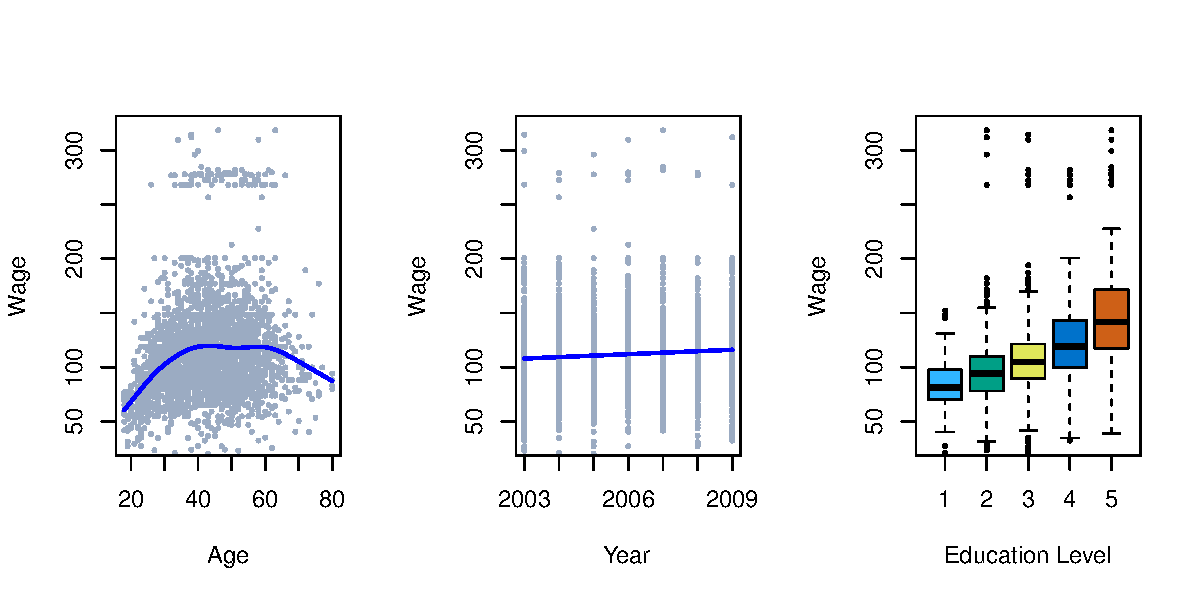
\includegraphics[width=\textwidth]{Figures_Chapters_1-6/Chapter1/1_1.pdf} \\
\scriptsize Source: ISLR2 Figure 1.1
\end{frame}

\begin{frame}{Classification}
  \begin{itemize}
     \item Predicts \textbf{categorical} or \textbf{qualitative} output values
     \item Model quality measured by proportion of mis-classification
  \end{itemize}
\centering
\vspace{5mm}
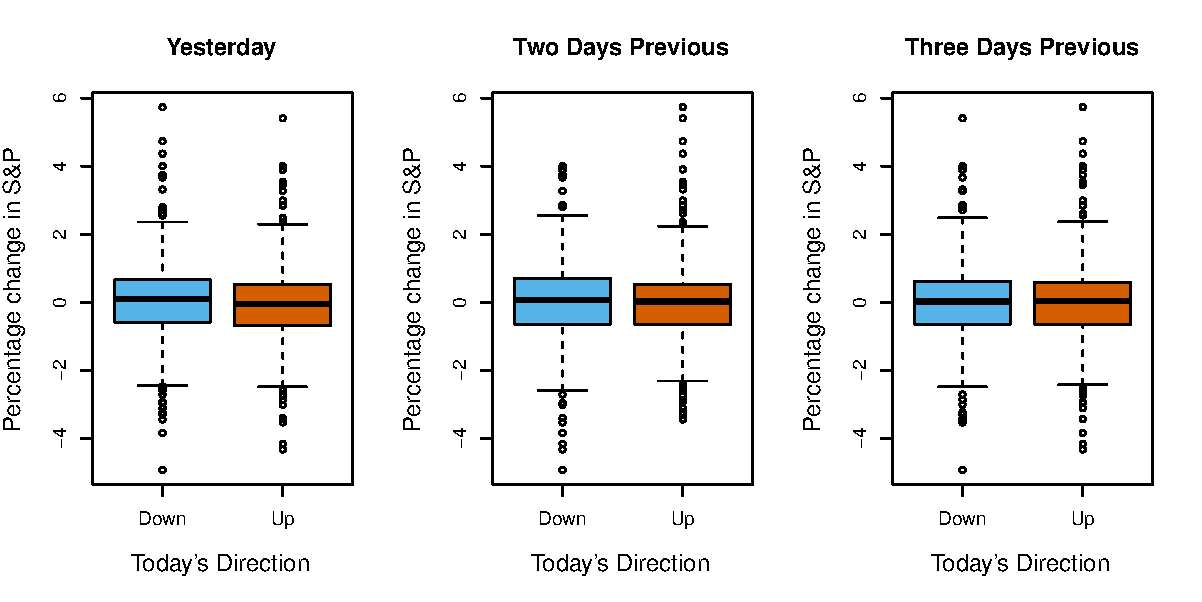
\includegraphics[width=\textwidth]{Figures_Chapters_1-6/Chapter1/1_2.pdf}
\scriptsize Source: ISLR2 Figure 1.2
\end{frame}

\begin{frame}{Regression Methods -- Examples}
\begin{block}{Parametric Methods}
\begin{itemize}
   \item \textbf{Linear Regression}
   \item \textbf{Ridge and Lasso Regression}
   \item Principal components regression
   \item Non-linear regression
\end{itemize}
\end{block}

\begin{block}{Non-Parametric Methods}
\begin{itemize}
  \item \textbf{K-Nearest-Neighbours (KNN)}
  \item Regression trees
  \item Smoothing splines
  \item Multivariate adaptive regression splines
  \item Kernel regression
\end{itemize}
\end{block}
\end{frame}

\begin{frame}{Classification Methods -- Examples}
\begin{itemize}
   \item Decision trees
   \item Random forests
   \item Bayesian networks
   \item Support vector machines
   \item Neural networks
   \item \textbf{Logistic regression}
   \item \textbf{Naive Bayes}
   \item Probit model
   \item Genetic programming
   \item \textbf{K-Nearest-Neighbours (KNN)}
\end{itemize}
\end{frame}

\begin{frame}{Prediction and Explanation}
\begin{block}{Explanation}
  \begin{itemize}
     \item Identifying causal mechanisms
     \item Testing causal hypotheses or explanations
     \item \emph{Inference} to \emph{population parameters} (points, intervals)
     \item Form of relationship between inputs and outputs is important (parsimony, ease of interpretation)
  \end{itemize}
\end{block}

\begin{block}{Prediction}
  \begin{itemize}
     \item Predict outputs for new observations
     \item Point or interval predictions, predictive distributions
     \item Focus on specific observations/cases
     \item Form of relationship between inputs and outputs is not important (may be complex, difficult to interpret)
  \end{itemize}
\end{block}
\end{frame}

\begin{frame}{Prediction and Explanation \small [cont'd]}
\begin{center}
\renewcommand{\arraystretch}{1.25}

\begin{tabular}{c|c} \hline
\textbf{Explanation} & \textbf{Prediction} \\ \hline
Causation & Association \\
Theory & Data \\
Retrospective & Prospective \\
Bias & Variance \\ \hline
\end{tabular}
\end{center}
\vspace{5mm}
\small{Based on: Shmueli, G. (2010). To Explain or To Predict?. Statistical Science, 25, 289-310.}
\end{frame}

\section{Regression}

\begin{frame}{Hands-On Exercises}
For each of the following problems, decide if it is a prediction or inference/explanation problem:
\begin{enumerate}
   \item How do real estate prices vary with location and age?
   \item What is the most important predictor of real estate prices?
   \item What is the expected sales price for a house at 310 Elizabeth Ave?
   \item Is the month of the sale an important predictor of real estate prices?
   \item Calculate the difference in expected sales prices for the house at 310 Elizabeth Avenue when sold in August and February
   \item When should a house be sold to achieve the best price?
\end{enumerate}
\end{frame}

\begin{frame}{Model Quality --- Regression}
\begin{itemize}
   \item MSE (mean squared error) or MAE (mean absolute error)
\end{itemize}
\begin{align*}
MSE = \frac{1}{n}\sum_{i=1}^n (y_i - \hat{f}(x_i))^2 \qquad \qquad
MAE = \frac{1}{n}\sum_{i=1}^n |y_i - \hat{f}(x_i)|
\end{align*}
\begin{itemize}
   \item Evaluation focus is on unseen test data, not training data
   \begin{itemize}
      \item Train on past stock market info, but predict future stock performance
      \item Train on previous patient info, but predict future patient outcomes
      \item Train on past real estate prices, but predict future prices
   \end{itemize}
   \item \emph{Separate \textbf{training data} from \textbf{test data} to evaluate model quality (''holdout sample'')}
   \item Low training error does NOT imply low testing error
\end{itemize}
\end{frame}

\begin{frame}{Quality of Fit}{Between model and data}
\begin{block}{Degrees of Freedom}
\begin{itemize} 
  \item How much a function can be adapted to fit training data
  \item Number of independently (''freely'') adjustable parameters
\end{itemize}
\end{block}

\centering
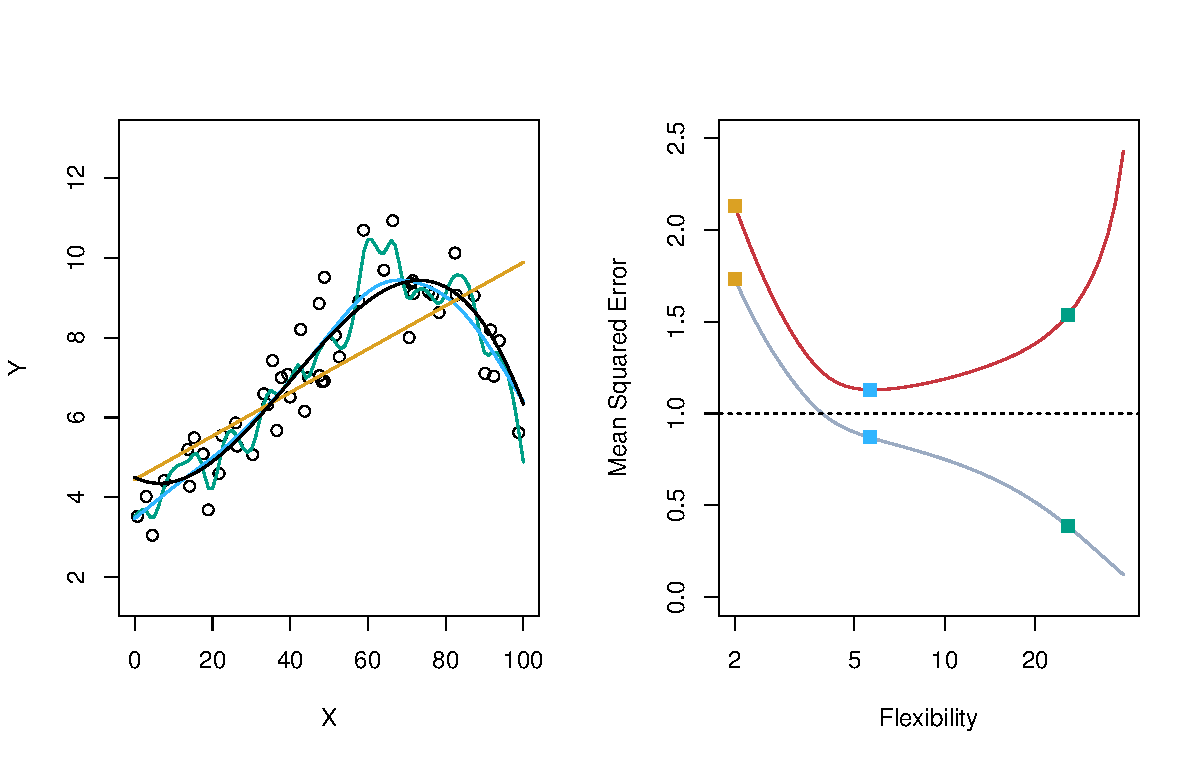
\includegraphics[width=.9\textwidth]{Figures_Chapters_1-6/Chapter2/2_9.pdf} \\

\scriptsize Source: ISLR2 Fig 2.9
\end{frame}


\begin{frame}{Quality of Fit \small [cont'd]}
\begin{block}{Overfitting}
  \begin{itemize}
     \item Small training error
     \item Large testing error
     \item Model exploits random idiosyncrasies of the data set
  \end{itemize}
\end{block}

\begin{block}{Underfitting}
  \begin{itemize}
     \item Large training error
     \item Large testing error
     \item Model is insufficiently able to fit true pattern in data (too simple, inflexible)
  \end{itemize}
\end{block}
\end{frame}

\begin{frame}{Overfitting with Polynomial Expansions}
\centering
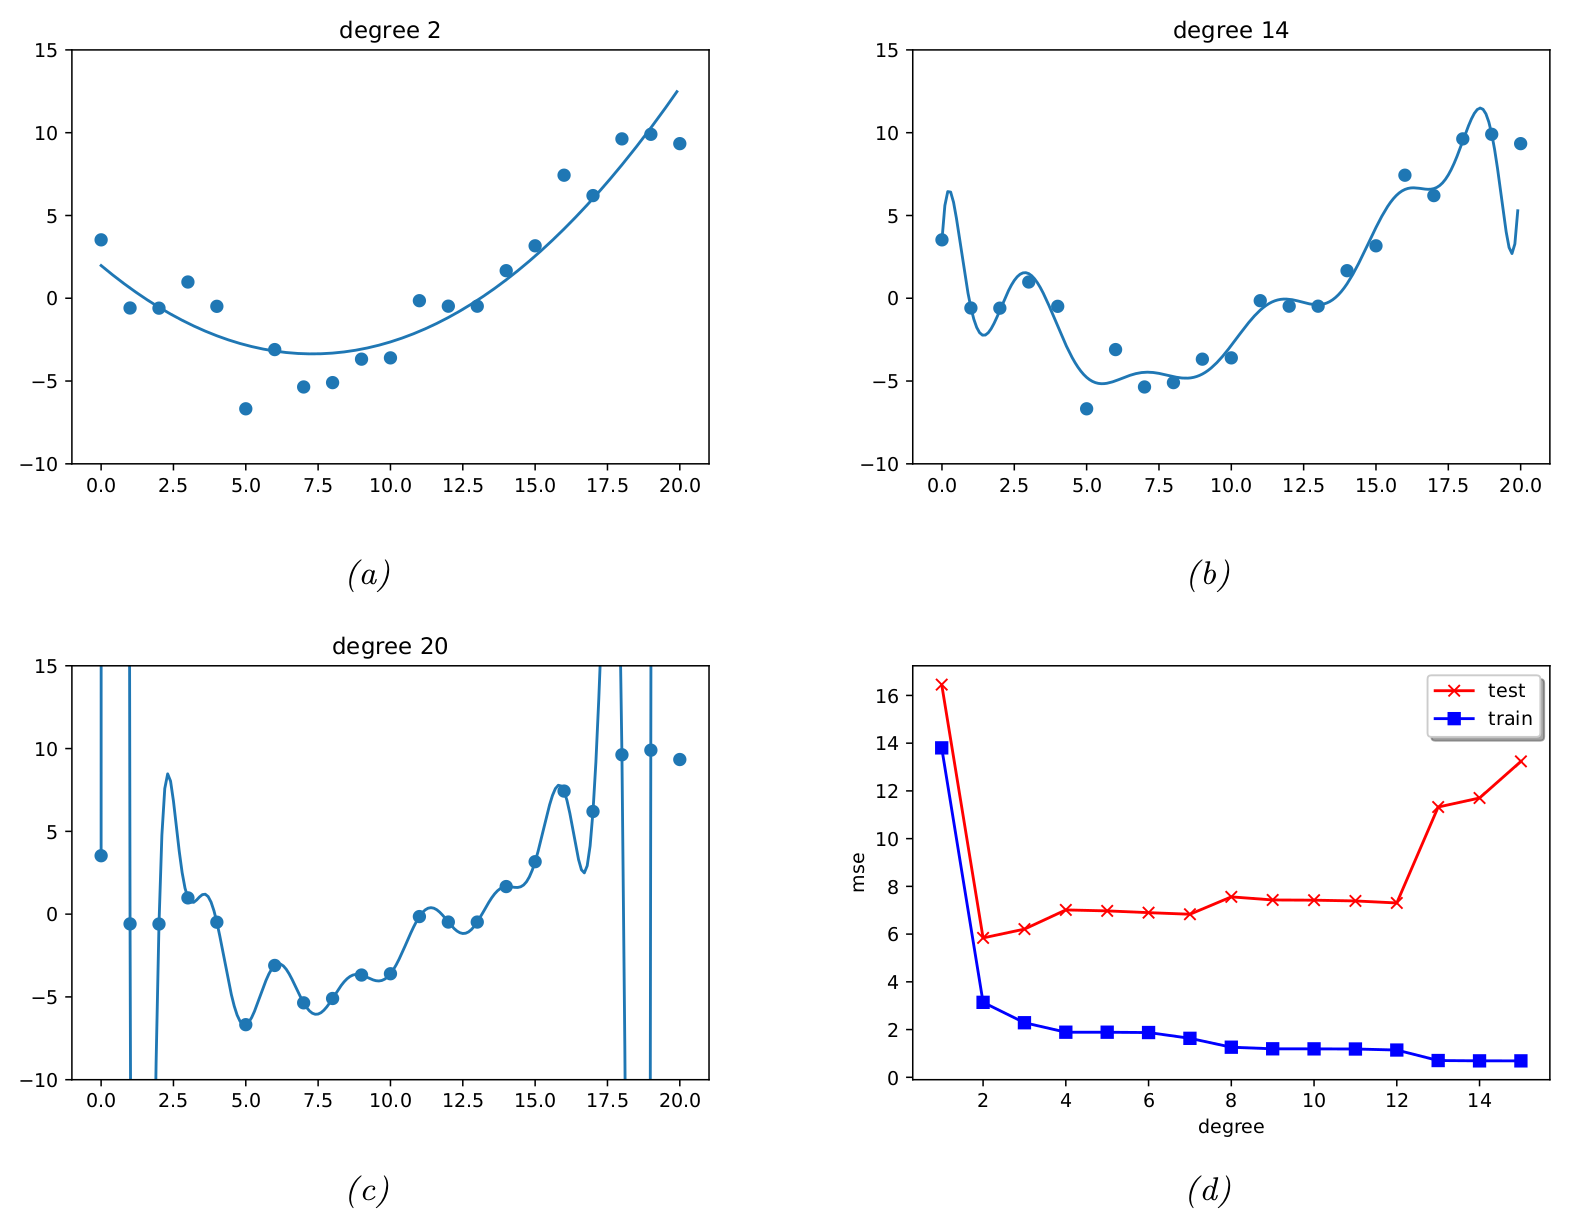
\includegraphics[width=.9\textwidth]{screen2.png} \\

\scriptsize Source: Murphy Figure 1.7
\end{frame}


\begin{frame}{Bias and Variance}
\begin{block}{Recall: Expected Value}
\begin{align*}
E[X] &= \sum_{i=1}^{\infty} x_i p_i \qquad \text{discrete random variable}\\
E[X] &= \int_{-\infty}^{\infty} x f(x) dx \qquad \text{continuous random variable}
\end{align*}
(for uniform distributions or unweighted observations $p_i=p_j \; \forall i, j \; $ so that $E[X] = \frac{1}{n} \sum_{i=1}^{\infty} x_i $, i.e. expectation = mean)
\end{block}

\begin{block}{Recall: Variance}
\begin{align*}
Var[X] &= E[(X - E[X])^2] = E[X^2] - E[X]^2 
\end{align*}
(for zero-centered variables $E[X] = 0$ so that $Var[X] = E[X^2]$)
\end{block}
\end{frame}

\begin{frame}{Bias and Variance Decomposition \\ \small Example using mean squared error loss}
\begin{align*}
MSE &= E[(y - \hat{f})^2] &\qquad (\text{unweighted})\\
    & = E [ y^2 - 2 y \hat{f} + \hat{f}^2] \\
    &= E [y^2] - 2E[y\hat{f}] + E[\hat{f}^2] \\
\\
E[\hat{f}^2] &= E[\hat{f}^2] - E[\hat{f}]^2 + E[\hat{f}]^2 \\
             &= Var[\hat{f}] + E[\hat{f}]^2 \\
\\             
E[y^2] &= E[(f+\epsilon)^2] \\
       &= E[f^2] + 2E[f \epsilon] + E[\epsilon^2]\\
       &= f^2 + 2f \cdot 0 + \sigma^2 &\qquad (f \text{\, is not random and} \, E[\epsilon] = 0)\\
       &= f^2 + \sigma^2 \\ 
\end{align*}
\end{frame}

\begin{frame}{Bias and Variance Decomposition \small [cont'd] \\ \small Example using mean squared error loss}
\begin{align*}
E[y \hat{f}] &= E[(f + \epsilon)\hat{f}] \\
             &= E[f \hat{f}] + E[\epsilon \hat{f}] \\
             &= E[f \hat{f}] + E[\epsilon] E[\hat{f}] \\
             &= E[f \hat{f}] + 0 \cdot E[\hat{f}] \\
             &= f E[\hat{f}] \\
\\
MSE &= f^2 + \sigma^2 - 2 f E[\hat{f}] + Var[\hat{f}] + E[\hat{f}]^2 \\
    &= (f - E[\hat{f}])^2 + \sigma^2 + Var[\hat{f}] \\
    &= Bias[\hat{f}]^2 + \sigma^2 + Var[\hat{f}] \\
\end{align*}
\end{frame}

\begin{frame}{Bias and Variance Trade-Off}
\centering
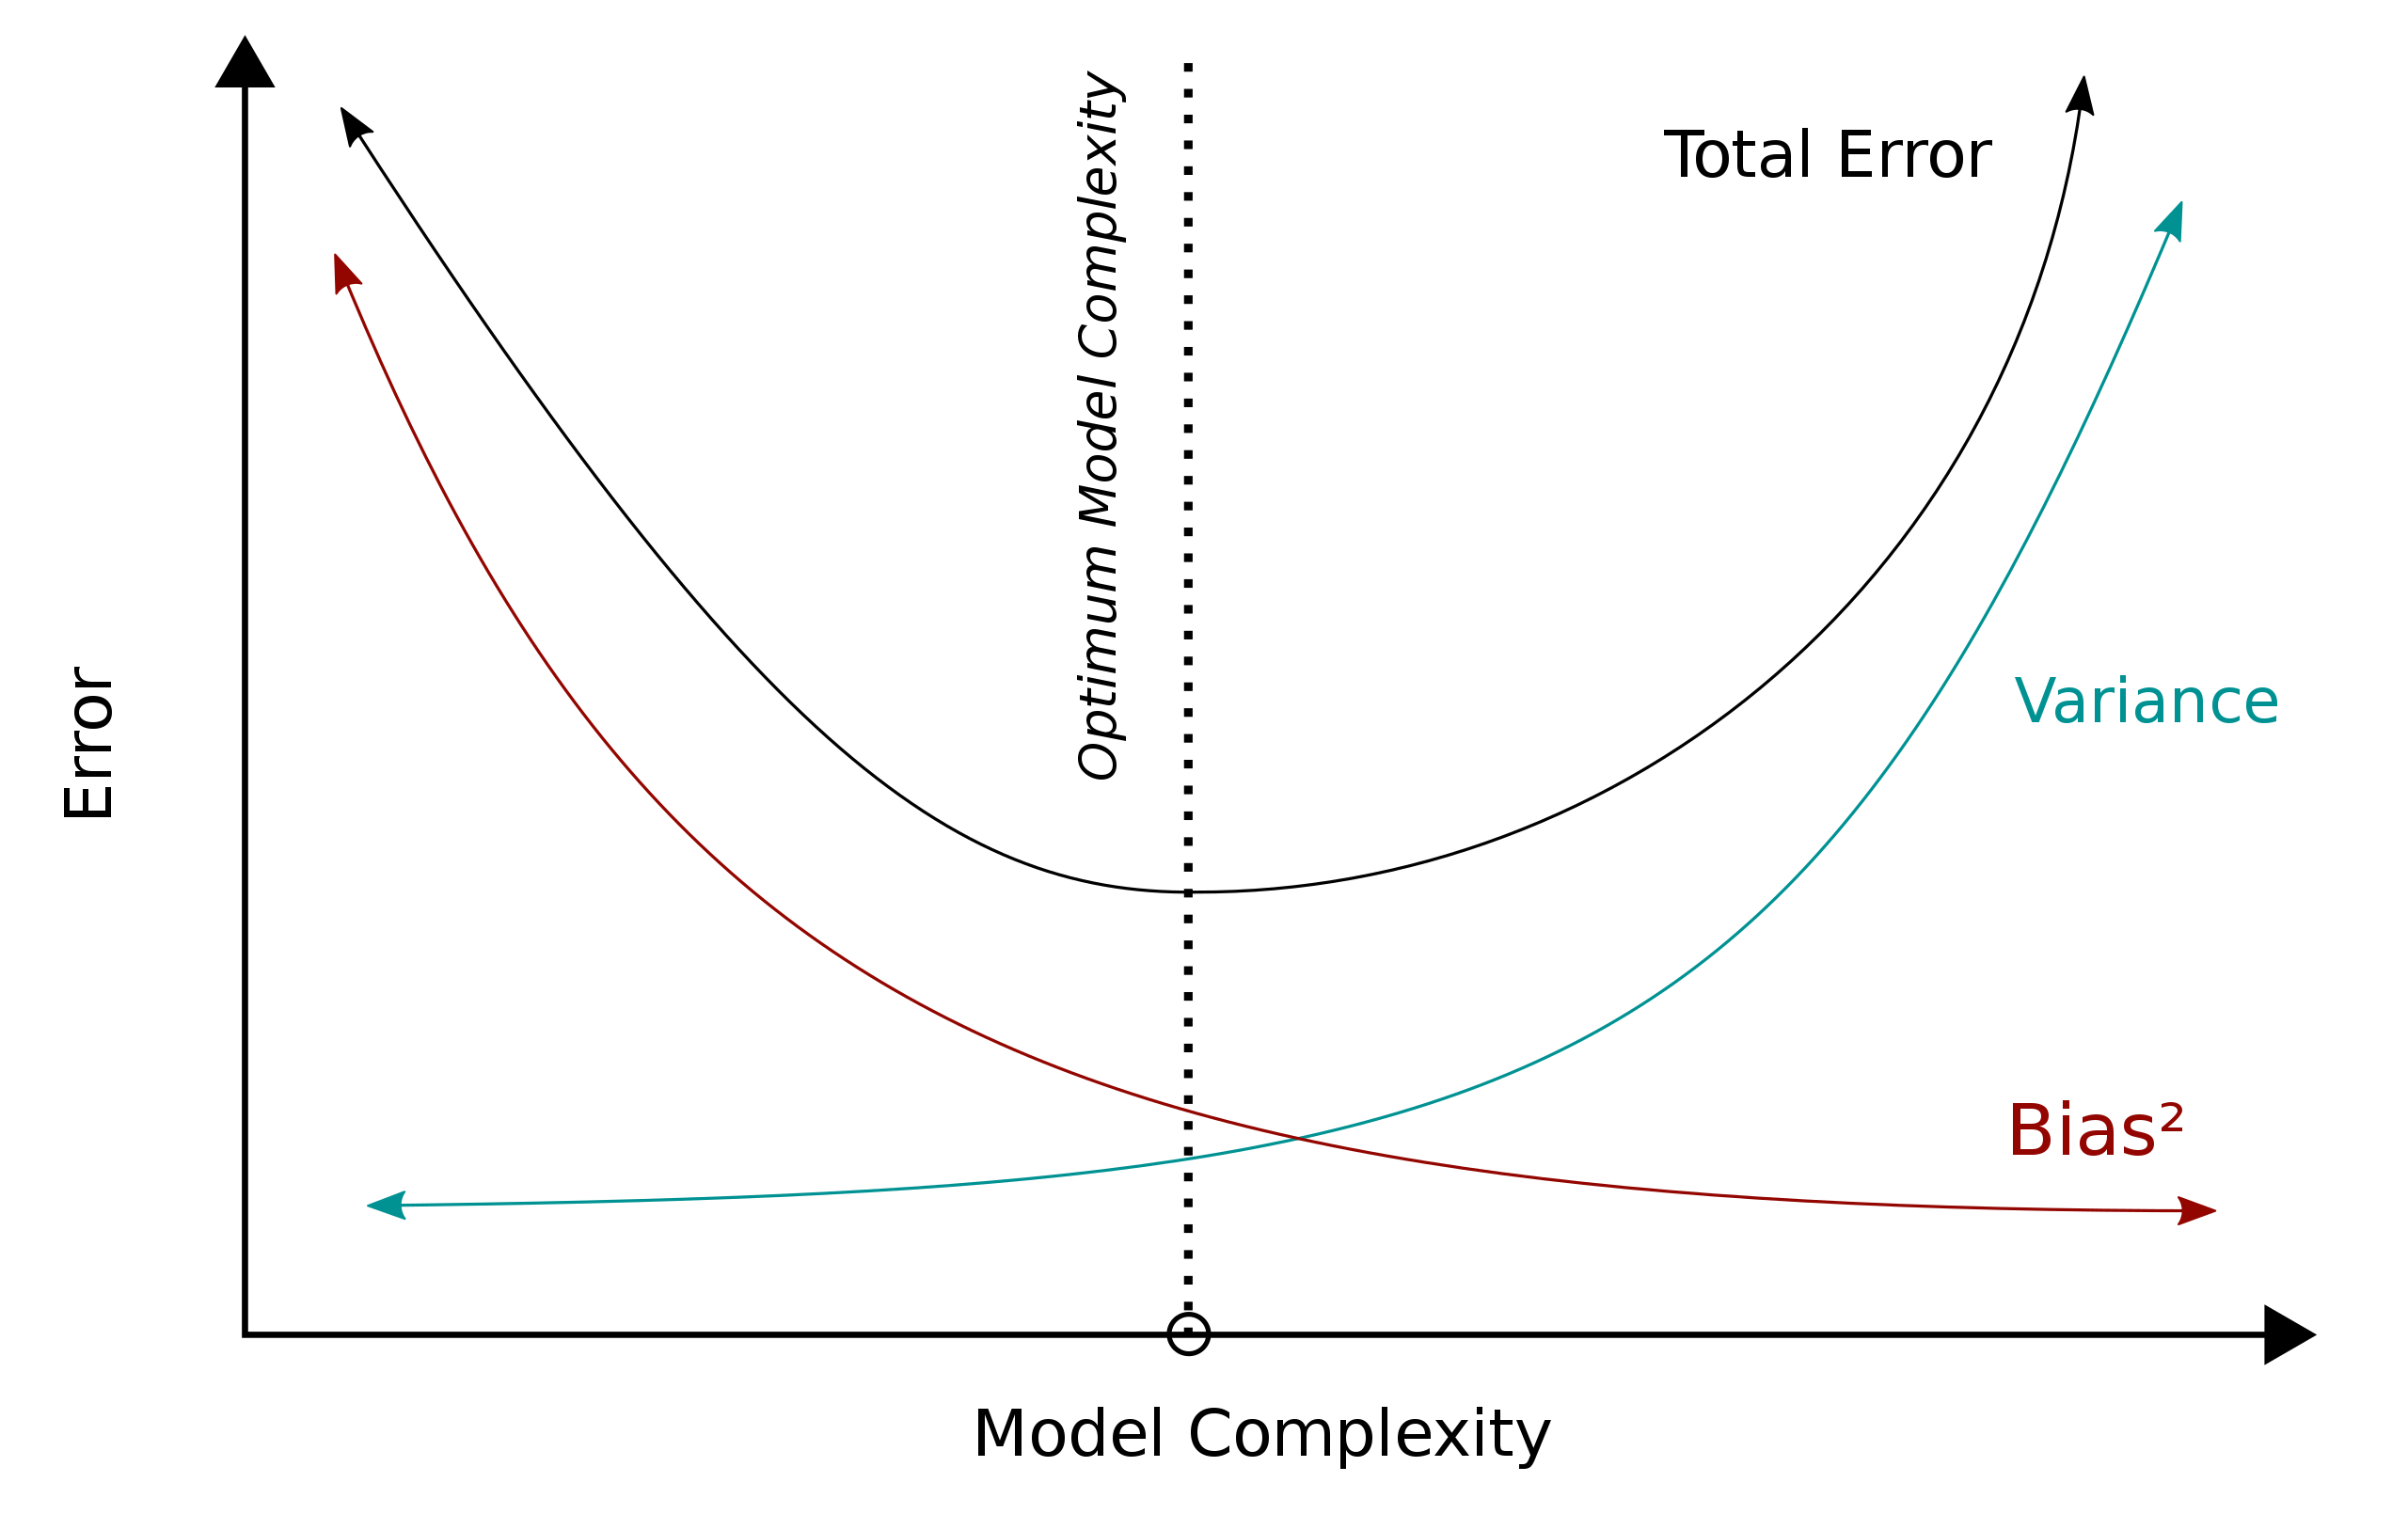
\includegraphics[width=\textwidth]{bias_variance.png}\\

\scriptsize \url{https://commons.wikimedia.org/wiki/File:Bias_and_variance_contributing_to_total_error.svg}
\end{frame}

\begin{frame}{Bias and Variance Trade-Off}
\begin{block}{Bias}
  \begin{itemize}
     \item Model (assumptions) error
     \item $Bias[\hat{f}]$ is the error introduced by a wrong/simplified model
     \item \textbf{High bias}: Model is too simple to represent true relationship $\rightarrow$ \textbf{Underfitting}
   \end{itemize}
\end{block}
\begin{block}{Variance}
  \begin{itemize}
     \item Training data error due to model complexity 
     \item $Var[\hat{f}]$ is the variability between training data sets (samples)
     \item \textbf{High variance}: Model is too complex and exploits random noise in training data $\rightarrow$ \textbf{Overfitting}
  \end{itemize}
\end{block}
\end{frame}

\begin{frame}{Bias and Variance Trade-Off \small [cont'd]}
\begin{block}{Irreducible Error}
  \begin{itemize}
     \item Unmeasured variables
     \item Measurement error
     \item $\sigma^2$ cannot be predicted from $x_i$ so cannot be reduced.
  \end{itemize}
\end{block}
\end{frame}

\begin{frame}{Bias and Variance Trade-Off \small [cont'd]}
\begin{itemize}
  \item \emph{Explanation} focuses on bias reduction \\(i.e. find the ''true'' functional form)
  \item \emph{Prediction} focuses on variance reduction \\(functional form is irrelevant).
  \item High variance models are complex, but complex models need not have high variance.
  \item High bias (simple models) does not imply large prediction error
  \item Lower prediction error does not imply low bias (simple models)
\end{itemize}
\end{frame}

%\begin{frame}{Model Bias and Estimation Bias in Penalized Models}{Examples: Ridge Regression or LASSO}
%\begin{columns}
%\begin{column}{.33\textwidth}
%\textbf{Model Bias}: Error between best fitting approximation and true function \\
%\vspace{3mm}
%\textbf{Estimation Bias}: Error between average estimate and best-fitting approximation
%\end{column}
%\begin{column}{.66\textwidth}
%\begin{center}
%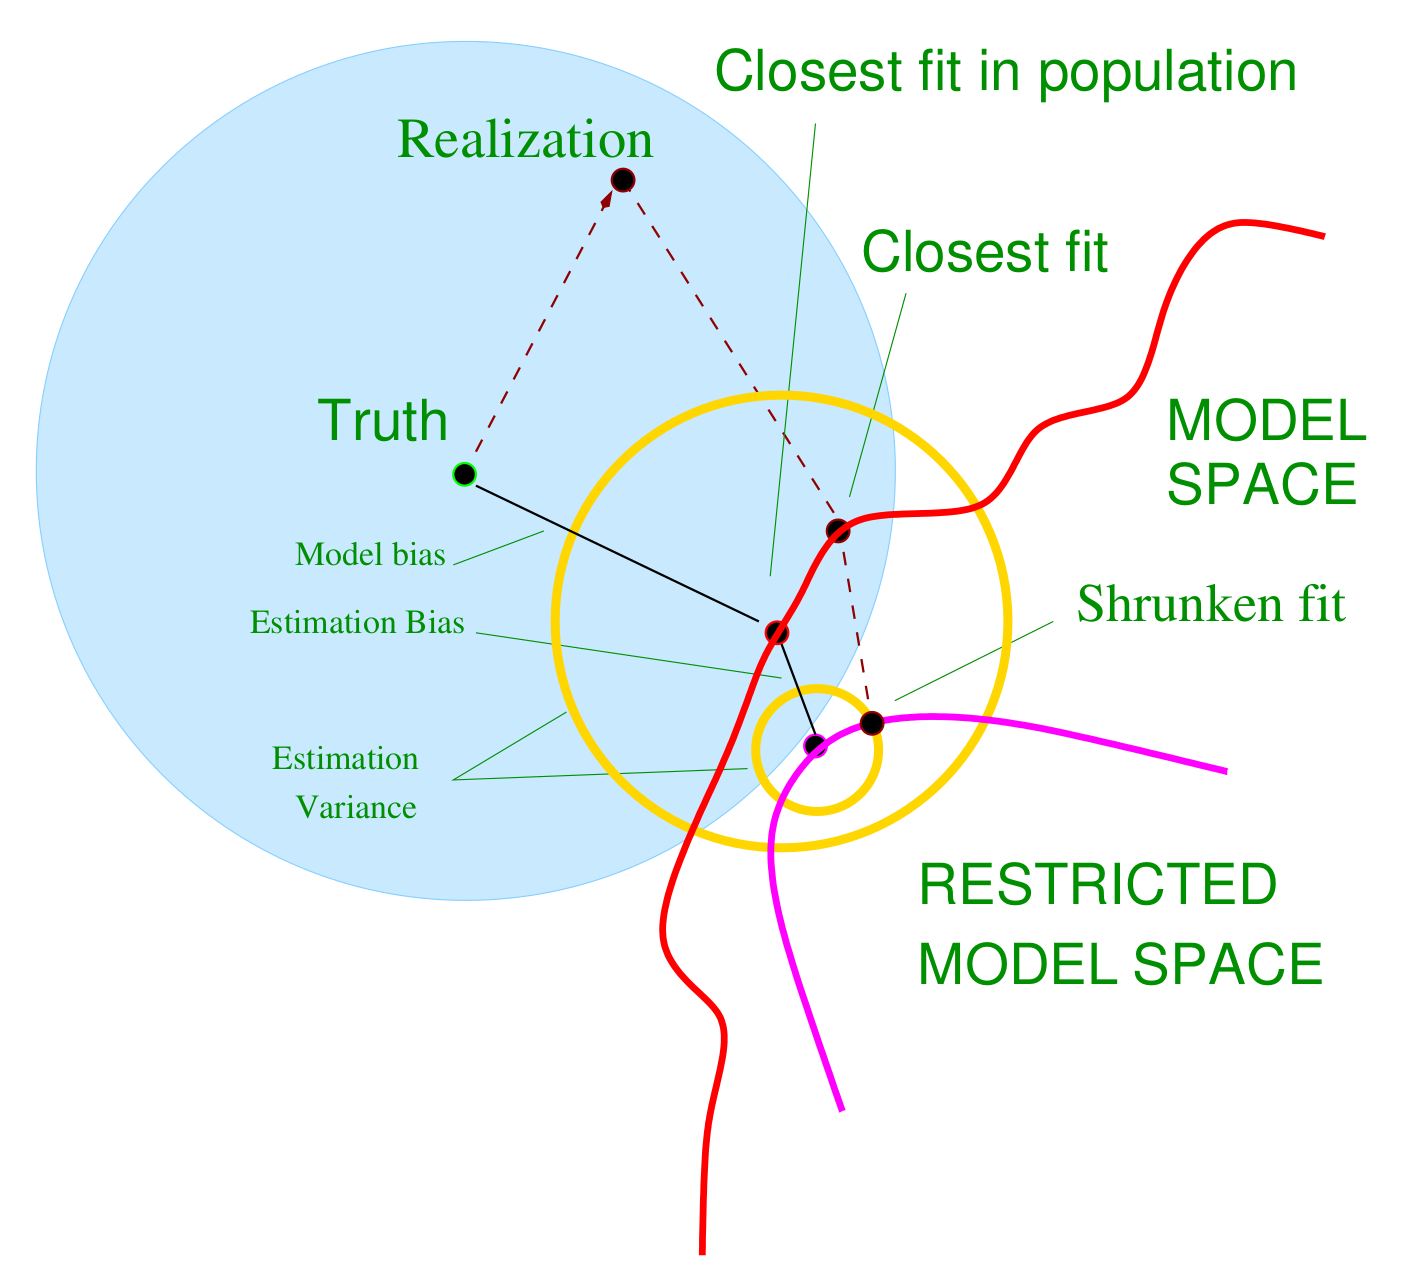
\includegraphics[width=\textwidth]{screen1.png} \\
%\scriptsize Source: ESL Figure 7.2
%\end{center}
%\end{column}
%\end{columns}
%\end{frame}

\begin{frame}{Review Questions -- Bias and Variance}
\begin{enumerate}
  \item Define bias and variance in the context of machine learning models.
  \item Explain the bias-variance tradeoff with an example. You may use a simple regression model as a reference.
  \item Describe a scenario where a high-bias model would be more appropriate than a low-bias model.
  \item Given the following scenarios, identify whether the model is likely suffering from high bias, high variance, or is well-balanced:
	\begin{itemize}
	  \item A model that performs well on training data but poorly on unseen test data.
	  \item A simple linear regression model that is unable to capture the complexities of the data, resulting in poor performance on both training and test data.
	  \item A model that performs equally well on training and test data.
	\end{itemize}
\end{enumerate}
\end{frame}

\begin{frame}{Review Questions -- Bias and Variance \small [cont'd]}
\begin{enumerate}
  \setcounter{enumi}{4}
  \item Describe techniques to reduce bias in a machine learning model.
  \item Given a dataset where the relationship between features and target is non-linear and complex, propose a strategy to improve a model that initially has high bias (e.g., linear regression).
  \item List and explain strategies to reduce variance in a machine learning model.
  \item Imagine you have a deep learning model that performs exceptionally well on the training data but poorly on the validation data. What steps would you take to address this issue?
\end{enumerate}
\end{frame}

\section{Classification}

\begin{frame}{Model Quality --- Classification}
\begin{block}{Error Rate}
\begin{align*}
\frac{1}{n}\sum^n_{i=1} \Ident(y_i \neq \hat{y}_i)
\end{align*}
\end{block}
\footnotesize
where $\Ident(\cdot)$ is the \emph{identity function} that is 1 if its argument is true, 0 otherwise.
\normalsize

\vspace{\baselineskip}
\begin{itemize}
  \item Training error rates
  \item Testing error rates
\end{itemize}
\end{frame}

\begin{frame}{Bayes Classifier}
\small
\begin{block}{Classifier}
Assign each observation to the most likely class given its predictor values
\begin{align*}
\argmax_j \Pr(Y=j| X=x_0)
\end{align*}
\end{block}

\begin{block}{Error Rate}
\begin{align*}
1 - E \left( \argmax_j \Pr (Y=j | X) \right)
\end{align*}
\end{block}
\end{frame}

\begin{frame}{Bayes Decision Boundary}

\centering
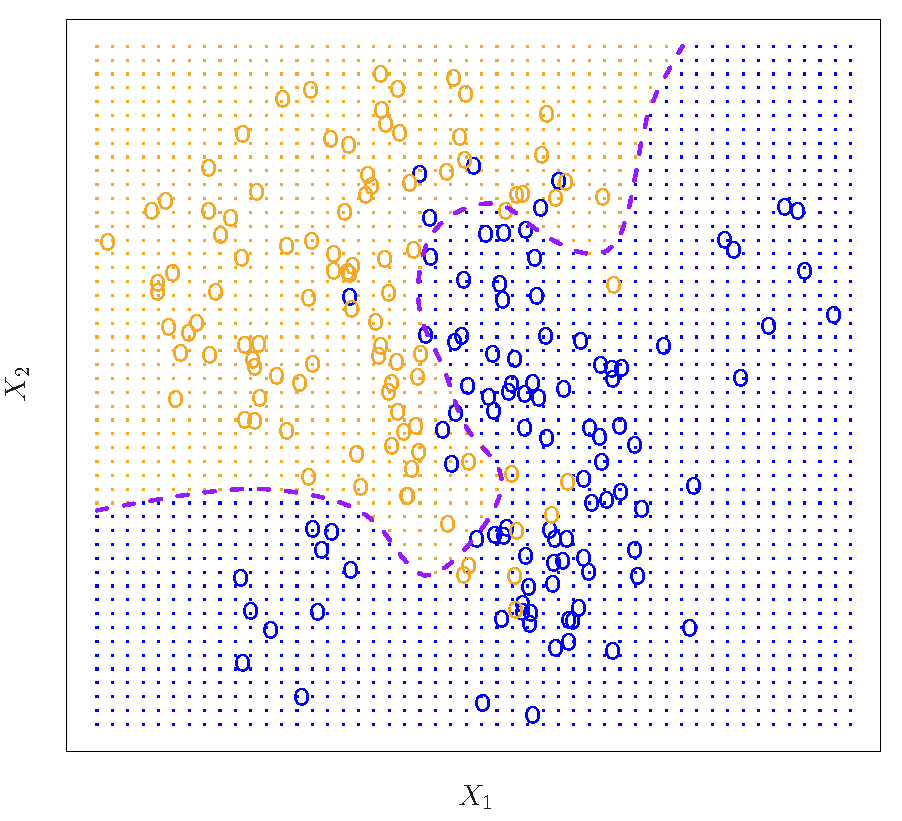
\includegraphics[height=2.75in]{Figures_Chapters_1-6/Chapter2/2_13.pdf} \\
\vspace{3mm}
\scriptsize Source: ISLR2 Figure 2.13
\end{frame}

\begin{frame}{Bayes Classifier \small [cont'd]}
\begin{itemize}
\item Bayes classifier is an \emph{ideal} classifier
\item Bayes error rate is lower bound, irreducible error
\item Conditional probabilities are unknown in practice
\item Estimation introduces error
\end{itemize}
\end{frame}


\begin{frame}{Example --- K-Nearest-Neighbour (KNN)}
\begin{itemize}
  \item Identify set of $K$ points closest to observation $x_0$ called $N_0$
\begin{align*}
\Pr (Y=j|X=x_0) = \frac{1}{K} \sum_{i \in N_0} \Ident (y_i=j) 
\end{align*}
where $\Ident(\cdot)$ is the identity function that is 1 if its argument is true, and 0 otherwise.
\end{itemize}
\begin{itemize}
   \item Classify in class of highest probability
\end{itemize}
\end{frame}

\begin{frame}{K=3}
\centering
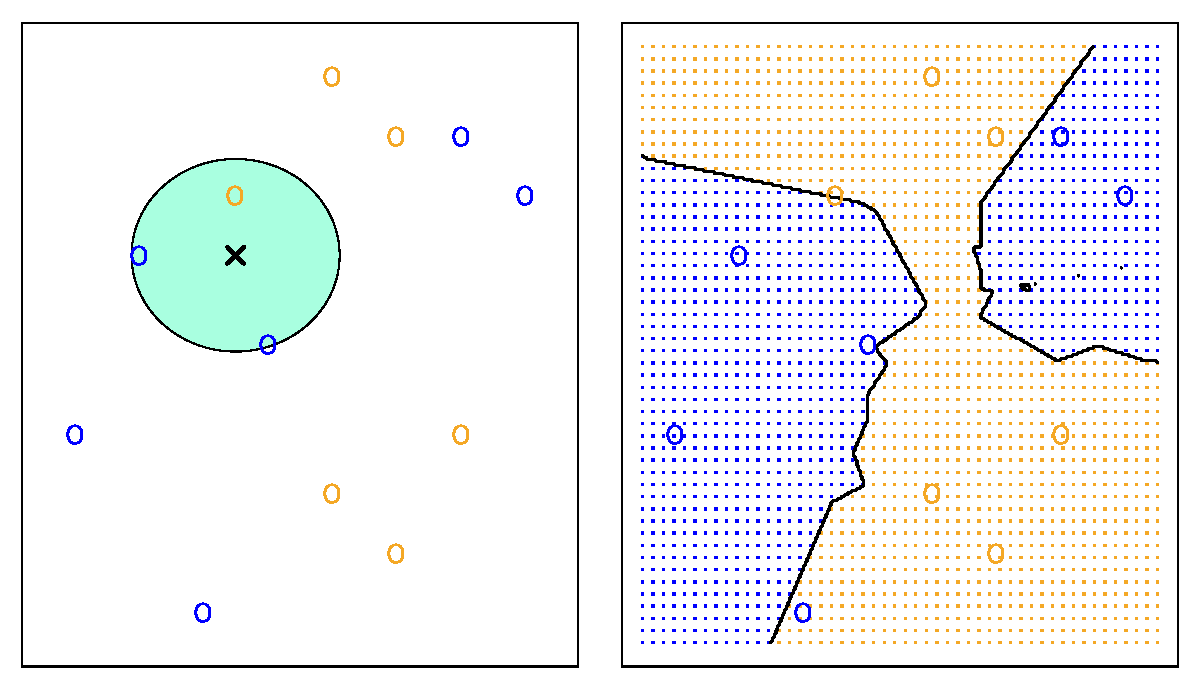
\includegraphics[width=\textwidth]{Figures_Chapters_1-6/Chapter2/2_14.pdf} \\
\vspace{3mm}
\scriptsize Source: ISLR2 Figure 2.14
\end{frame}

\begin{frame}{KNN and Bayes Classifier}
\centering
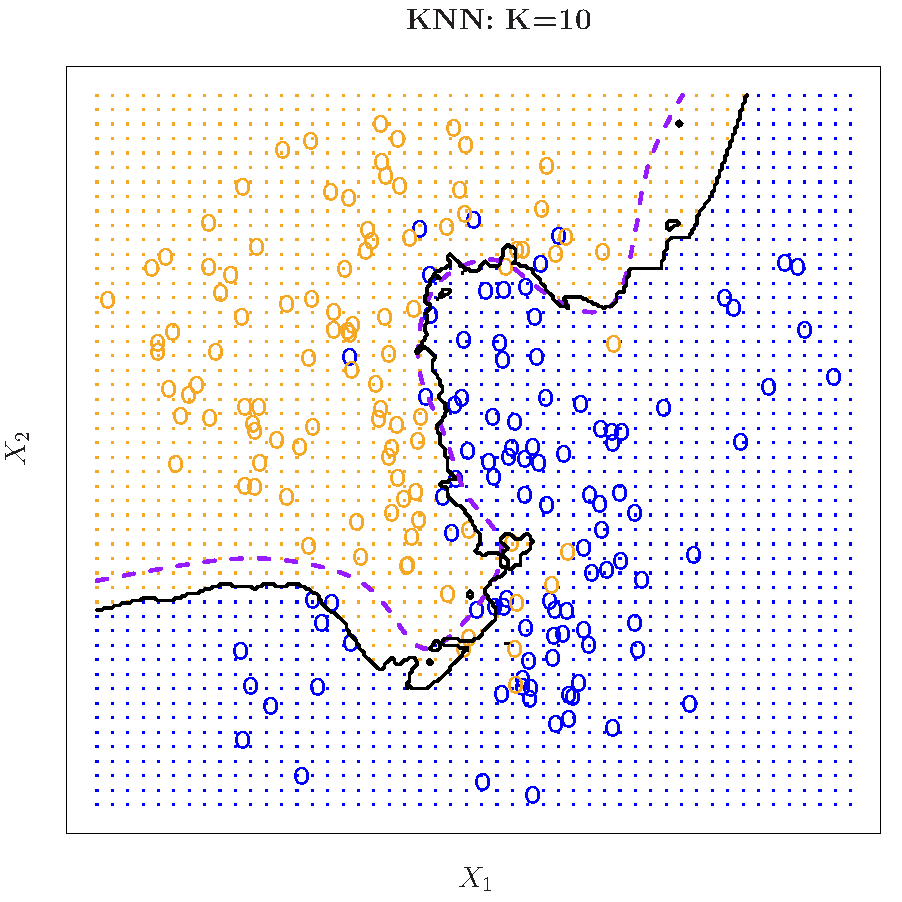
\includegraphics[height=2.75in]{Figures_Chapters_1-6/Chapter2/2_15.pdf} \\
\vspace{3mm}
\scriptsize Source: ISLR Figure 2.15
\end{frame}

\begin{frame}{KNN Quality}
\centering
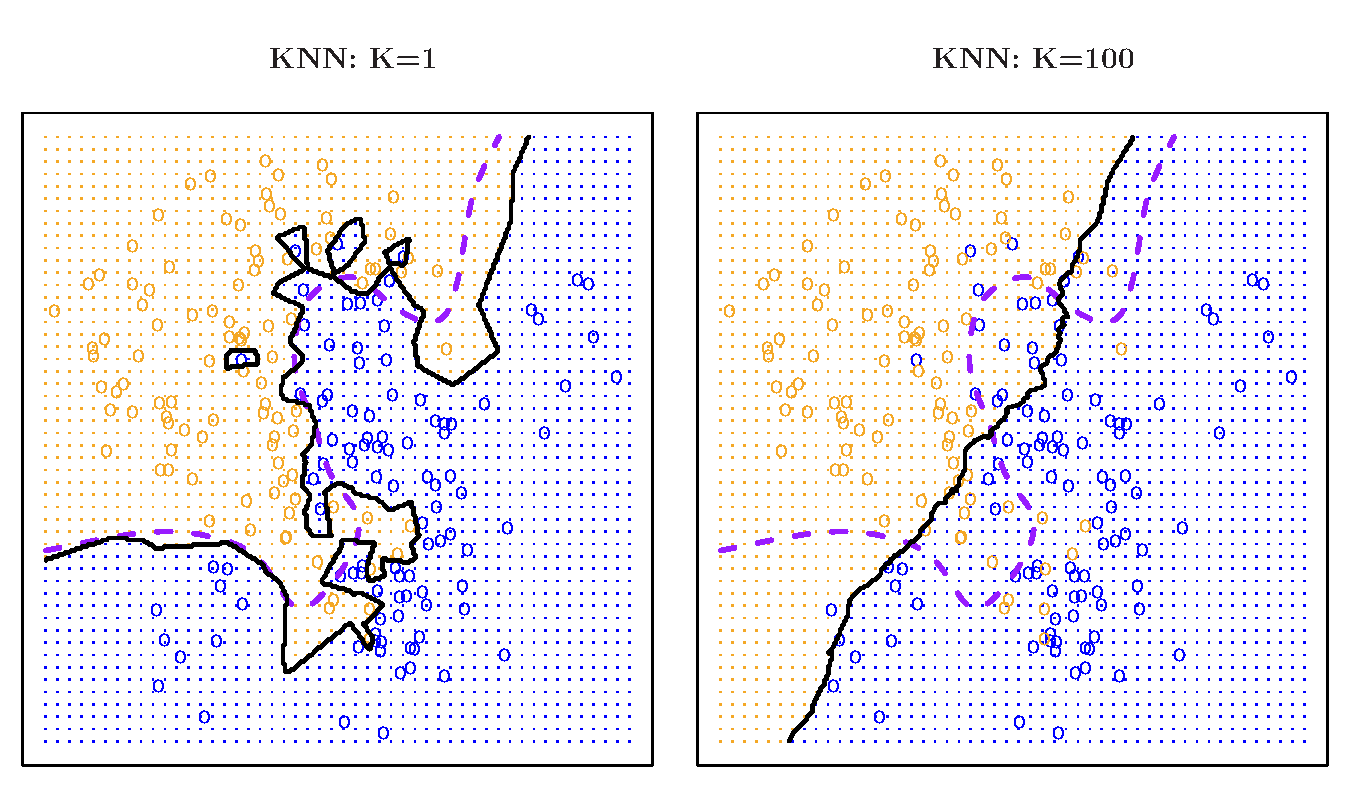
\includegraphics[width=\textwidth]{Figures_Chapters_1-6/Chapter2/2_16.pdf} \\
\vspace{3mm}
\scriptsize Source: ISLR2 Figure 2.16
\end{frame}

\begin{frame}{KNN Error Rates}
\centering
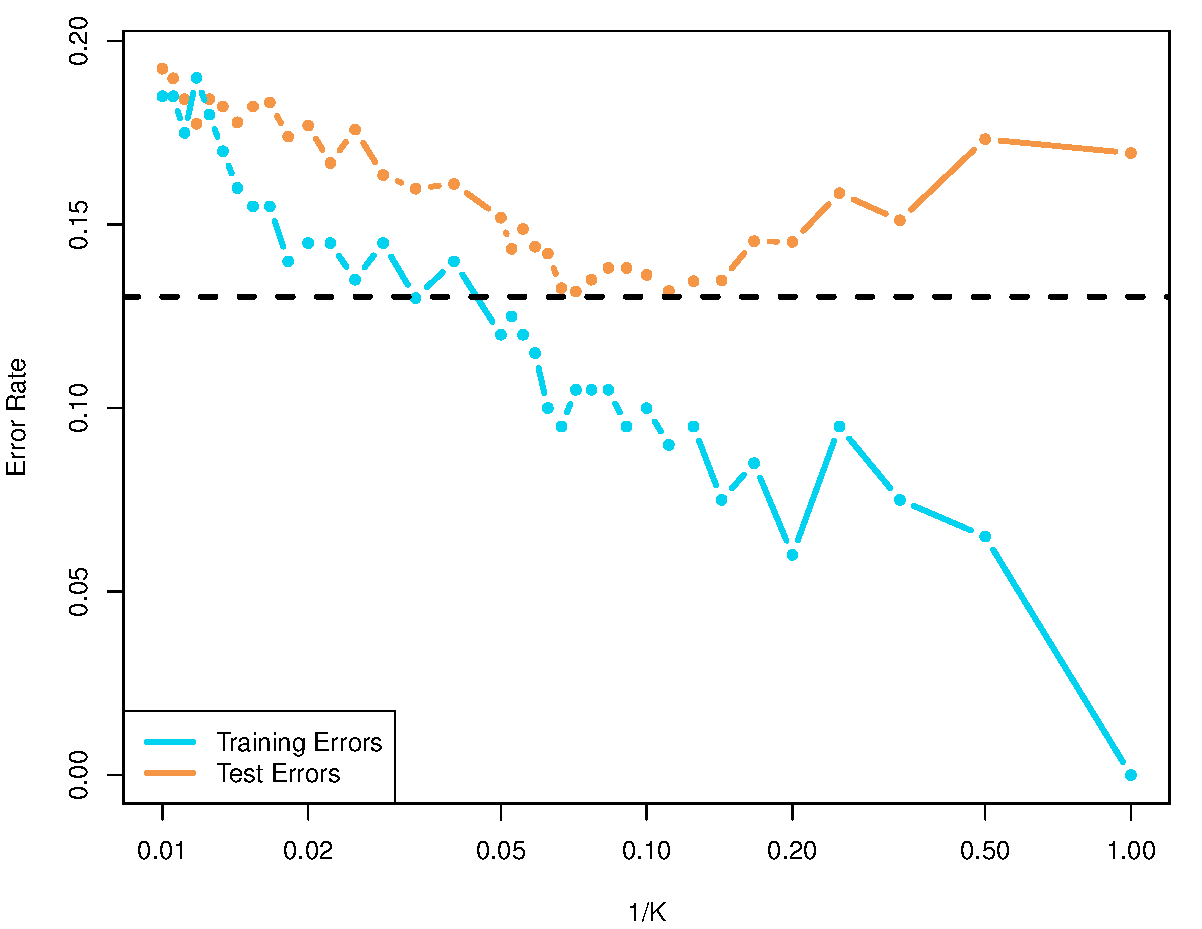
\includegraphics[width=.8\textwidth]{Figures_Chapters_1-6/Chapter2/2_17.pdf} \\
\vspace{3mm}
\scriptsize Source: ISLR2 Figure 2.17
\end{frame}

\begin{frame}{Hands-On Exercise -- KNN}
\small
The table below provides a training data set containing six observations, three predictors, and one qualitative response variable

\begin{center}
\footnotesize
%\renewcommand{\arraystretch}{1.25}
\begin{tabular}{l|r|r|r|l} \hline
Obs. & $X_1$ & $X_2$ & $X_3$ & $Y$ \\ \hline
1 & 0 & 3 & 0 & Blue \\
2 & 2 & 0 & 0 & Blue \\
3 & 0 & 1 & 3 & Blue \\
4 & 0 & 1 & 2 & Yellow \\
5 & -1 & 0 & 1 & Yellow \\
6 & -1 & 1 & 1 & Blue \\ \hline
\end{tabular}
\end{center}

Suppose we wish to use this data set to make a prediction for $Y$ when $X_1=X_2=X_3=0$ using K-nearest neighbours.

\begin{enumerate}
  \item Compute the Euclidean distance (''l2-norm'') between each observation and the test point
  \item What are your prediction with $K=1$? With $K=3$? Why?
  \item If the Bayes decision boundary is highly non-linear, would you expect the best value for K to be large or small? Why?
\end{enumerate}

\scriptsize Adapted from ISLR Exercise 2.7
\end{frame}


\begin{frame}{Binary Classification Model Quality --- Confusion Matrix}

\begin{block}{}
\begin{center}
\renewcommand{\arraystretch}{1.25}

$\Pr(\text{default=Yes} | X=x) > 0.5$ (Bayes) \\ \vspace{2mm}
\begin{tabular}{cc|cc|c} \hline
     & & \multicolumn{2}{c|}{\emph{True default status}} \\
     & & No & Yes & Total \\ \hline
\emph{Predicted} & No & 9644 & \emph{252} & 9896 \\ 
\emph{default status} & Yes & \emph{23} & 81 & 104 \\ \hline
     & Total & 9667 & 333 & 10000 \\ \hline
\end{tabular} \\
\end{center}
\scriptsize Source: ISLR2 Table 4.4
\end{block}

\begin{itemize}
  \item Overall error rate: 2.75\%
  \item Of the defaulters, only $24.3\%$ were correctly predicted (\textbf{''sensitivity''}) ($81/333$), error rate $75.7\%$
  \item Of the non-defaulters, $99.8\%$ were correctly predicted (\textbf{''specificity''}), error rate $0.02\%$
\end{itemize}
\end{frame}

\begin{frame}{Confusion Matrix -- Adjusting Thresholds \small [cont'd]}
\begin{block}{}
\begin{center}
\renewcommand{\arraystretch}{1.25}

$\Pr(\text{default=Yes} | X=x) > 0.2$ \\ \vspace{2mm}
\begin{tabular}{cc|cc|c} \hline
     & & \multicolumn{2}{c|}{\emph{True default status}} \\
     & & No & Yes & Total \\ \hline
\emph{Predicted} & No & 9432 & 138 & 9570 \\ 
\emph{default status} & Yes & 235 & 195 & 430 \\ \hline
     & Total & 9667 & 333 & 10000 \\ \hline
\end{tabular} \\
\end{center}

\scriptsize Source: ISLR2 Table 4.5
\end{block}

\begin{itemize}
  \item Overall error rate: 3.73\% 
  \item Sensitivity = 58.6\%;
  \item Specificity = 97.6\%
\end{itemize}
\end{frame}

\begin{frame}{Confusion Matrix \small [cont'd]}
\begin{block}{}
\small
\begin{center}
\renewcommand{\arraystretch}{1.25}

\begin{tabular}{cc|cc|c} \hline
     & & \multicolumn{2}{c|}{\emph{True class}} \\
     & & No (-) & Yes (+) & Total \\ \hline
\emph{Predicted} & No (-) & True Neg. (TN) & False Neg. (FN) & $N^*$ \\ 
\emph{class} & Yes (+) & False Pos. (FP) & True Pos. (TP) & $P^*$ \\ \hline
     & Total & $N$ & $P$ &  \\ \hline
\end{tabular} \\
\end{center}
\end{block}
\end{frame}

\begin{frame}{Binary Classification Model Quality}
\begin{itemize}
   \item Sensitivity, \textbf{Recall}, Hit Rate, True Positive Rate
\begin{align*}
TPR = \frac{TP}{P} = \frac{TP}{TP+FN} = 1 - FNR
\end{align*}
   \item \textbf{Specificity}, Selectvitity, True Negative Rate
\begin{align*}
TNR = \frac{TN}{N} = \frac{TN}{TN+FP} = 1 - FPR
\end{align*}
   \item \textbf{Precision}, Positive Predictive Value
\begin{align*}
PPV = \frac{TP}{TP+FP} = 1 - FDR
\end{align*}
   \item Negative Predictive Value
\begin{align*}
NPV = \frac{TN}{TN+FN} = 1 - FOR
\end{align*}
\end{itemize}
\end{frame}

\begin{frame}{Binary Classification Model Quality \small [cont'd]}
\begin{itemize}
   \item Miss Rate, False Negative Rate
\begin{align*}
FNR = \frac{FN}{P} = \frac{FN}{FN + TP} = 1 - TPR
\end{align*}
   \item Fall-out, False Positive Rate
\begin{align*}
FPR = \frac{FP}{N} = \frac{FP}{FP+TN} = 1 - TNR
\end{align*}
   \item False Discovery Rate
\begin{align*}
FDR = \frac{FP}{FP+TP} = 1 - PPV
\end{align*}
   \item False Omission Rate
\begin{align*}
FOR = \frac{FN}{FN+TN} = 1 - NPV
\end{align*}
\end{itemize}
\end{frame}      

\begin{frame}{Binary Classification Model Quality \small [cont'd]}
\begin{itemize}
   \item \textbf{Accuracy} (= 1 - Error Rate)
\begin{align*}
ACC = \frac{TP+TN}{P+N} = \frac{TP + TN}{TP + TN + FP + FN}
\end{align*}
   \item \textbf{F1 Score} (harmonic mean of precision and recall)
\begin{align*}
F1 = 2 \times \frac{PPV \times TPR}{PPV + TPR} = \frac{2 TP}{2TP + FP + FN}
\end{align*}
   \item False Discovery Rate
\begin{align*}
FDR = \frac{FP}{FP+TP} = 1 - PPV
\end{align*}
   \item False Omission Rate
\begin{align*}
FOR = \frac{FN}{FN+TN} = 1 - NPV
\end{align*}
\end{itemize}
\end{frame}      

\begin{frame}{Binary Classification Model Quality \small [cont'd]}
\large ROC: Receiver Operating Characteristic \\

\normalsize
\centering
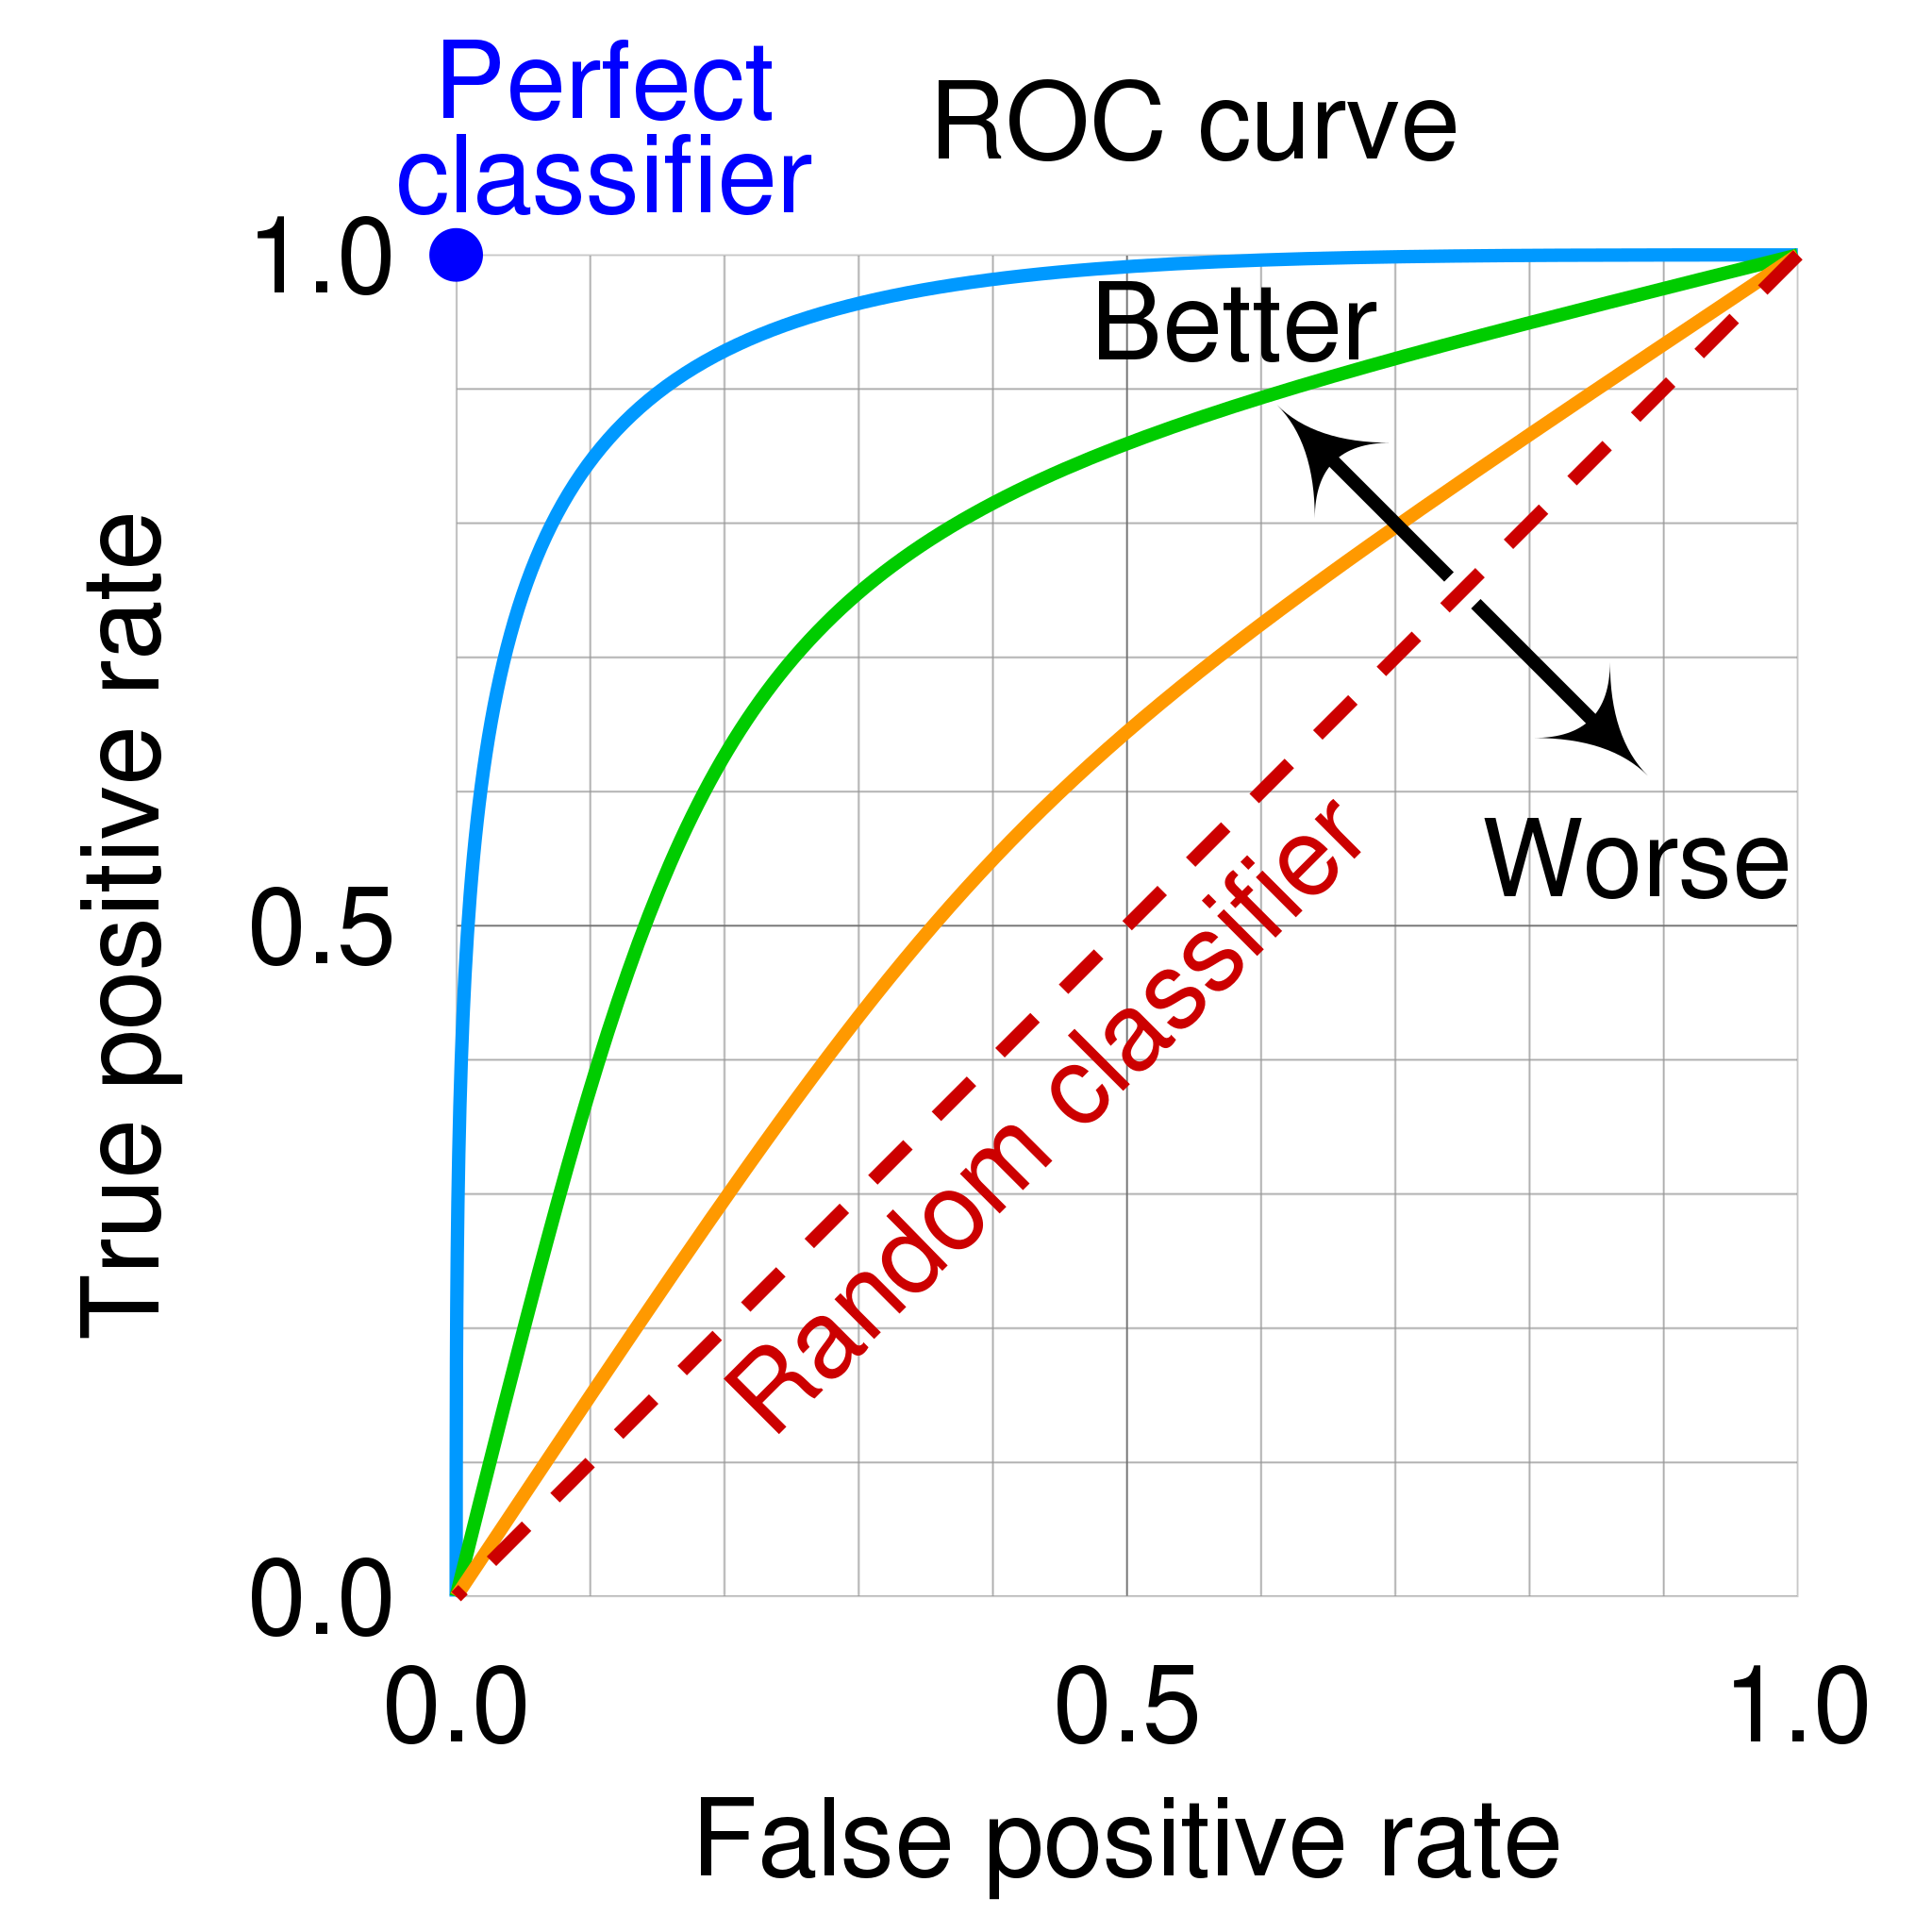
\includegraphics[height=2.5in]{roc.png}
\scriptsize \url{https://commons.wikimedia.org/wiki/File:Roc_curve.svg}
\end{frame}

\begin{frame}{Binary Classification Model Quality \small [cont'd]}
\large AUC: Area Under (ROC) Curve \\

\normalsize
\centering
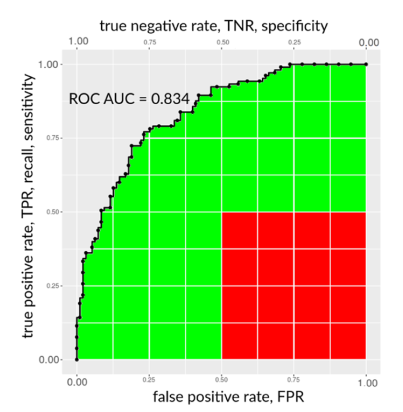
\includegraphics[height=2.5in]{auc.png}
\scriptsize \url{https://commons.wikimedia.org/wiki/File:ROC_curve_example_highlighting_sub-area_with_low_sensitivity_and_low_specificity.png}
\end{frame}

\begin{frame}{Hands-On Exercise -- Basic Calculations}
\begin{enumerate}
  \item Compute Precision and Recall for the two confusion matrixes above
  \item Computer Accuracy and F1 values for the two confusion matrixes above
  \item Plot the two points for this classifier in an ROC space/diagram. Are they above or below the diagonal?
\end{enumerate}
\end{frame}

%\begin{frame}{Hands-On Exercise -- Real World Scenario}
%Consider a medical testing scenario where 1000 individuals are tested for a disease. The results are:
%\begin{itemize}
  %\item 100 people actually have the disease, and 900 do not.
  %\item Out of the 100 people with the disease, 90 are correctly identified as having it, but 10 are not detected.
  %\item Of the 900 people without the disease, 810 are correctly identified as not having it, but 90 are incorrectly identified as having the disease.
%\end{itemize}
%\vspace{\baselineskip}
%\emph{Calculate the precision, recall, sensitivity, and accuracy.} \\

\emph{Tip}: Write down the confusion matrix first.
\end{frame}

\begin{frame}{Hands-On Exercise -- Interpretation Challenge}
Given the following results from a machine learning model:
\begin{itemize}
  \item Precision: 0.75
  \item Recall: 0.60
  \item Accuracy: 0.80
\end{itemize}
\vspace{\baselineskip}
Answer the following questions:
\begin{enumerate}
  \item What percentage of identified positives are actually positive?
  \item What percentage of actual positives are identified by the model?
  \item What percentage of the total classifications were correct?
\end{enumerate}
\end{frame}

\begin{frame}{Hands-On Exercise -- Adjusting Thresholds}
Consider a binary classification task with the following confusion matrix at a certain threshold:
\begin{itemize}
  \item TP: 150, FP: 50
  \item FN: 30, TN: 200
\end{itemize}
\vspace{\baselineskip}
\emph{Discuss how adjusting the classification threshold might affect precision, recall, and accuracy. What happens if the threshold is increased or decreased?}
\end{frame}

%\begin{frame}{Hands-On Exercise -- Base Rate Fallacy, Unbalanced Data}
%Imagine a rare disease called "Z-Disease" which affects only 1\% of the population. A pharmaceutical company has developed a test for Z-Disease that has the following characteristics:
%\begin{itemize}
  %\item Sensitivity (True Positive Rate): 95\% (i.e., the probability that if someone has Z-Disease, they will test positive).
  %\item Specificity (True Negative Rate): 90\% (i.e., the probability that if someone does not have Z-Disease, they will test negative).
%\end{itemize}
%Answer the following questions:
%\begin{enumerate}
  %\item What is the probability that a person who tests positive for Z-Disease actually has the disease?
  %\item Does the test's high sensitivity and specificity guarantee a reliable diagnosis? Why or why not?
%\end{enumerate}
%\end{frame}
 
\begin{frame}{Multi-Class Classification Model Quality}
\begin{block}{}
\small
\begin{center}
\renewcommand{\arraystretch}{1.25}

\begin{tabular}{cc|ccc|l} \hline
     & & \multicolumn{3}{c|}{\emph{True class}} \\
                 &   & 0 & 1 & 2 & Prob \\ \hline
\multirow{3}{1.1cm}{\emph{Predicted Class}} & 0 & 4 & 2 & 0 & $q_0 = 6/24  = .25$ \\ 
                 & 1 & 1 & 5 & 2 & $q_1 = 8/24  = .33$ \\
                 & 2 & 2 & 0 & 8 & $q_2 = 10/24 = .42$ \\ \hline
     & Prob & $p_0$ & $p_1$ & $p_2$ &  \\
     &      & $=7/24$ & $=7/24$ & $=10/24$ &  \\ 
     &      & $=.29$ & $=.29$ & $=.42$ &  \\ \hline
\end{tabular} \\
\end{center}
\end{block}
\begin{itemize}
   \item \textbf{Overall Accuracy}: sum(diag(.)) / sum(.) $=17/24=.71$
\end{itemize}
\end{frame}

\begin{frame}{Multi-Class Classification Model Quality}
\begin{block}{Reduction to Binary Classification}
\begin{itemize}
  \item ''One vs. Rest'' (OvR), ''One vs. All'' (OvA), ''One against All'' (OaA)
  \item Consider each class in turn as ''positive'' class, consider all others as ''negative'' class
\end{itemize}
\end{block}
\end{frame}

\begin{frame}{Multi-Class Classification Model Quality \small [cont'd]}
\begin{block}{Micro-Averaging}
\begin{itemize} 
  \item Count and sum TP, FP, FN over all classes
  \item Use the total TP, FP, FN to calculate Precision and Recall
\end{itemize}
\end{block}

\begin{itemize}
  \item Gives equal weight to each instance
  \item May overemphasize performance of a majority class when it dominates the data set
\end{itemize}

\begin{quote} \large
For multi-class classification, micro-average precision equals micro-average recall and equals accurary
\end{quote}
\end{frame}

\begin{frame}{Multi-Class Classification Model Quality \small [cont'd]}
\begin{block}{Macro-Averaging}
\begin{itemize} 
  \item Calculate precision and recall for each class (OvR)
  \item Average precision and recall, optionally weighting each class by its true count of instances
\end{itemize}
\end{block}

\begin{itemize}
   \item Appropriate when all classes are equally important
   \item Appropriate for imbalanced data sets so all classes contribute
   \item May mask poor performance on important minority classes
   \item May lower overall performance due to low performance on small or unimportant classes
\end{itemize}
\end{frame}

\begin{frame}{Hands-On Exercises}
For the multi-class confusion matrix above,
\begin{enumerate}
  \item Compute precision and recall for each class
  \item Compute the macro-averages of precision and recall
  \item Compute the micro-averages of precision and recall and show that they equal the accuracy
\end{enumerate}
\end{frame}

\begin{frame}{Multi-Class Classification Model Quality \small [cont'd]}
\begin{itemize}
  \item Dissimilarity between two probability distributions (information theoretic motivation)
  \begin{itemize}
     \item True probability distribution over classes $p_i$
     \item Predicted probability distribution over classes $q_i$
  \end{itemize}
  \item \textbf{Cross-entropy}: 
\begin{align*}
H(p, q) = - \sum_i p_i \log q_i
\end{align*}
  \item \textbf{Kullback-Leibler (KL) divergence}:
\begin{align*}
D_{KL}(P || Q) &= \sum_i p_i \log \left( \frac{p_i}{q_i} \right) \\
  & = \sum_i p_i \log p_i - \sum_i p_i \log q_i \\
  & = - H(p, p) + H(p, q)
\end{align*}
\end{itemize}
\end{frame}

\begin{frame}{Hands-On Exercises -- Cross-Entropy \& KL Divergence}
\begin{center}
\vspace{-3mm} \tiny \url{https://commons.wikimedia.org/wiki/File:Kullback-Leibler_distributions_example_1.svg}
\normalsize
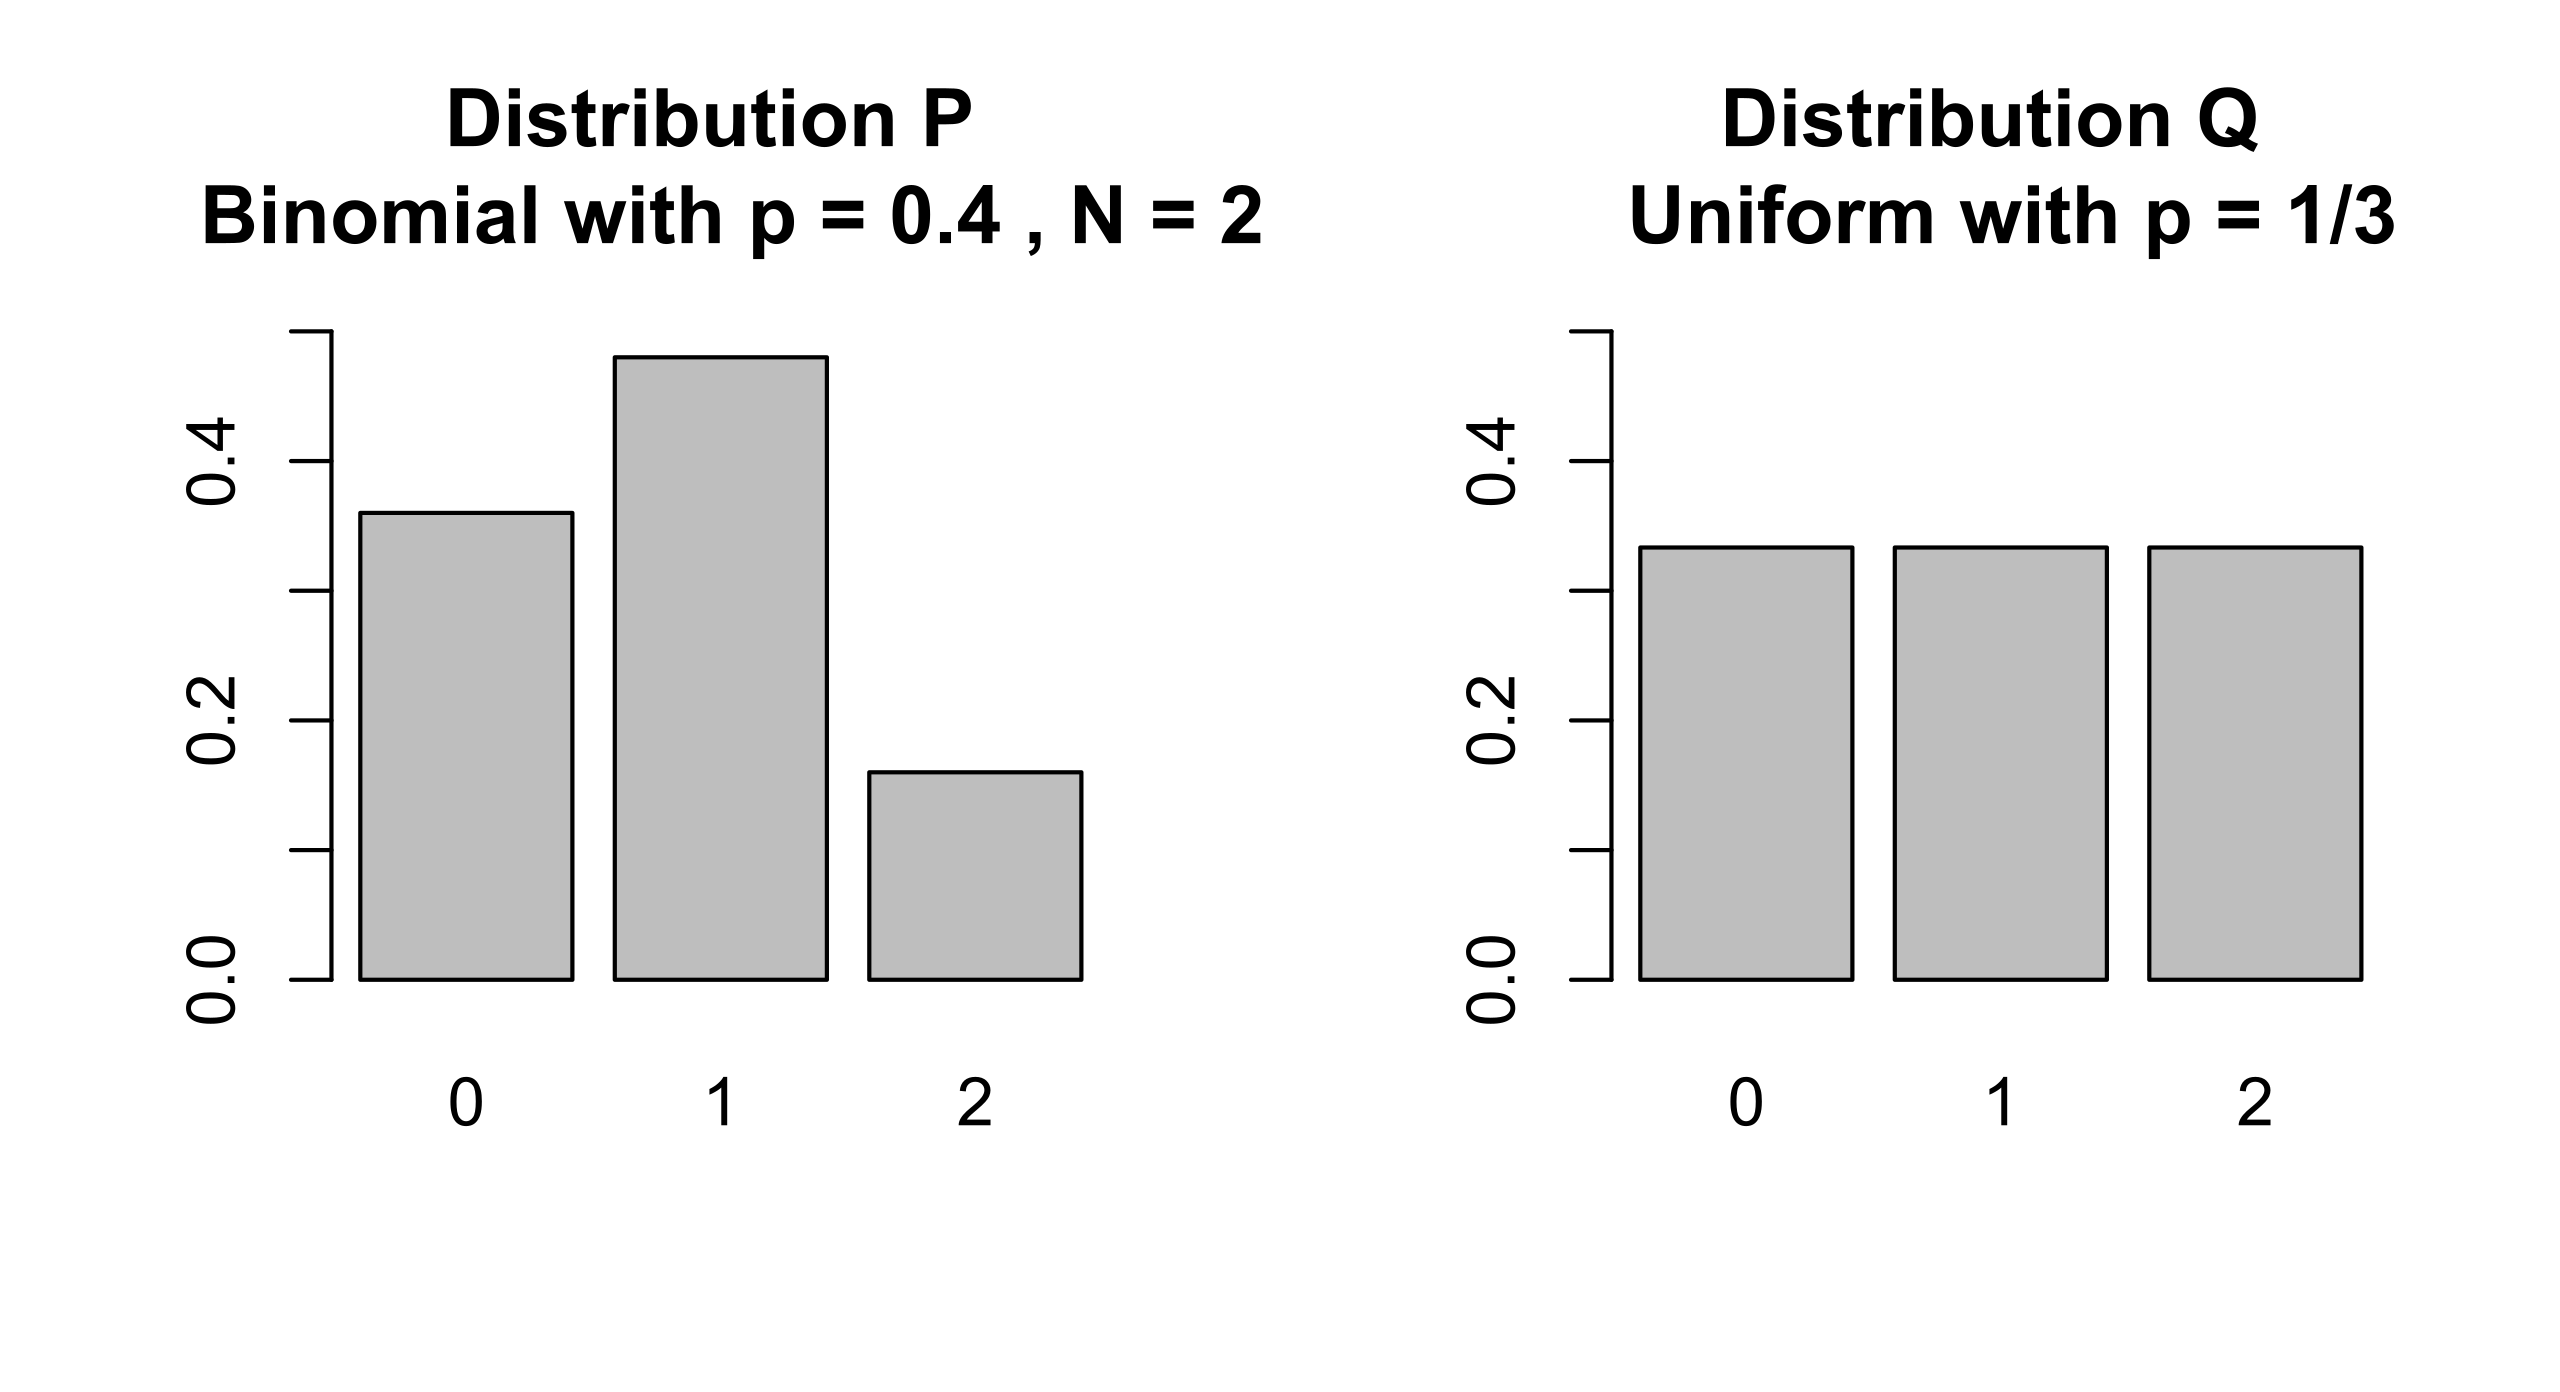
\includegraphics[width=.8\textwidth]{kl.png} \\
\end{center}

\vspace{-8mm}
\emph{Tip}: Binomial distribution: $\Pr(P=k) = \frac{n!}{k!(n-k)!} p^k (1-p)^{n-k}$ \\

%\vspace{3mm}
\begin{enumerate}
   \item Calculate the cross-entropy of P and Q
   \item Calculate the entropy of P
   \item Calculate the KL divergence of P and Q
\end{enumerate}
\end{frame}

\begin{frame}{Hands-On Exercises -- Cross-Entropy}
\begin{enumerate}
  \setcounter{enumi}{3}
  \item Calculate the cross-entropy and KL-divergence for the multi-class confusion matrix above
  \item Given two probability distributions P and Q over a discrete set of events, where $P = [0.1, 0.4, 0.5]$ and $Q = [0.2, 0.3, 0.5]$, calculate the cross-entropy $H(P, Q)$ and the KL-divergence $D_{KL}(P || Q)$.
\end{enumerate}
\end{frame}

\begin{frame}{Hands-On Exercise -- Cross-Entropy in Binary Classification}
In a binary classification task, you have the following probability distributions for the actual labels (P) and predicted labels (Q):
\begin{itemize}
  \item P = [1, 0] (the actual class is positive)
  \item Q = [0.7, 0.3] (the model predicts a 70\% chance of being positive)
\end{itemize}
\vspace{\baselineskip}
\emph{Calculate the cross-entropy loss for this scenario.}
\end{frame}

%\begin{frame}{Hands-On Exercise -- Kullback-Leibler Divergence}
%\begin{enumerate}
  %\item Calculate the KL divergence between the following probability distributions:
  %\begin{itemize}
     %\item P = [0.1, 0.9]
     %\item Q = [0.5, 0.5]
  %\end{itemize}
%\end{enumerate}
%\end{frame}

\begin{frame}{Hands-On Exercise -- KL Divergence in Practice}
Consider a scenario where you are comparing two models predicting weather conditions (sunny, cloudy, rainy). The actual distribution of weather conditions (P) and the predictions made by two models (Q1 and Q2) over a week are as follows:
\begin{itemize}
  \item P = [0.5, 0.3, 0.2]
  \item Q1 = [0.4, 0.4, 0.2]
  \item Q2 = [0.6, 0.2, 0.2]
\end{itemize}
\vspace{\baselineskip}
\begin{enumerate}
  \item Calculate the KL divergence for both models relative to the actual distribution.
  \item Which model is closer to the actual distribution based on the KL divergence?
\end{enumerate}
\end{frame}

\begin{frame}{Review Questions -- Cross-Entroy \& KL Divergence}
\begin{enumerate}
  \item Define cross-entropy and explain its significance in machine learning, especially in classification tasks.
  \item Discuss how cross-entropy can be used to evaluate the performance of a classification model.
  \item Define Kullback-Leibler divergence and explain its relationship with cross-entropy.
  \item Discuss how KL divergence is used in machine learning models, especially in the context of model optimization and feature selection.
\end{enumerate}
\end{frame}

\section{Resampling Methods}

\begin{frame}{Resampling Methods}
\begin{block}{Goals}
\begin{itemize}
  \item Unbiased assessment of true classification error
  \item Generalization to unseen values
\end{itemize}
\end{block}

\begin{block}{Model Selection}
Estimate the predictive performance (error) of different models in order to choose the best one
\end{block}

\begin{block}{Model Assessment}
Having chosen a final model, estimate is prediction error on new data (generalizability)
\end{block}
\end{frame}

\begin{frame}{Validation Set Approach (''Holdout'' Method)}
\begin{block}{Procedure}
\begin{itemize}
\item Randomly divide data:
\begin{itemize}
   \item \textbf{Training data}: Train each model
   \item \textbf{Validation data}: Test each trained model
   \item \textbf{Test data}: Evaluate the selected final model
\end{itemize}
\item Typical split: 50\% Training, 25\% Validation, 25\% Testing
\end{itemize}
\end{block}

\begin{block}{Characteristics}
\begin{itemize} 
  \item Validation error can be highly variable, depending on the split of data
  \item Validation error may overestimate actual error (bias), because of the smaller training set
\end{itemize}
\end{block}
\end{frame}

\begin{frame}{Validation Set Approach (''Holdout'' Method)}
\centering 

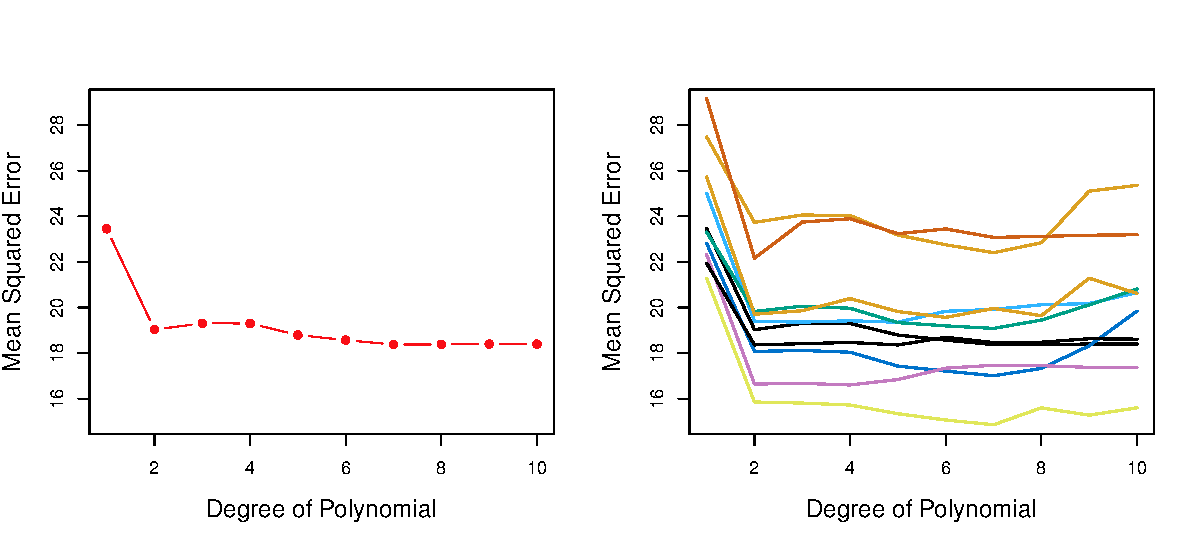
\includegraphics[width=\textwidth]{Figures_Chapters_1-6/Chapter5/5_2.pdf}
\scriptsize Source: ISLR2 Figure 5.2
\end{frame}

\begin{frame}{Leave One Out Cross-Validation (LOOCV)}
\begin{block}{Procedure}
\begin{enumerate}
\item Select one test observation
\item Train model with remaining $n-1$ observations
\item Test the trained model on selected test observation
\item Repeat steps 1--3 $n$ times with different test observations
\end{enumerate}
\begin{align*}
CV = \frac{1}{n} \sum\nolimits_{i=1}^n \operatorname{Err}_i
\end{align*}
\end{block}

\begin{block}{Characteristics}
\begin{itemize} 
  \item Computationally expensive
  \item Stable results, no randomness
  \item Less overestimation (bias) of error rate
\end{itemize}
\end{block}
\end{frame}

\begin{frame}{k-Fold Cross-Validation}
\begin{block}{Procedure}
\begin{enumerate}
\item Randomly divide data into $k$ sub-samples (''folds'')
\item Select one fold as test data
\item Train model on remaining $k-1$ folds
\item Test the trained model on test data fold
\item Repeat steps 2--4 $k$ times using each fold as test data
\end{enumerate}
\begin{align*}
CV = 1/k \sum\nolimits_{i=1}^k \operatorname{Err}_i
\end{align*}
\vspace{-\baselineskip}
\end{block}

\begin{block}{Characteristics}
\begin{itemize}
   \item Compromise between holdout method and LOOCV in terms of stability and computational expense
   \item Higher bias but lower variance of error estimate than LOOCV but lower variance than LOOCV
   \item \textbf{Typical $k=5$ to $k=10$}
\end{itemize}
\end{block}
\end{frame}

\begin{frame}{k-Fold Cross-Validation}
\centering

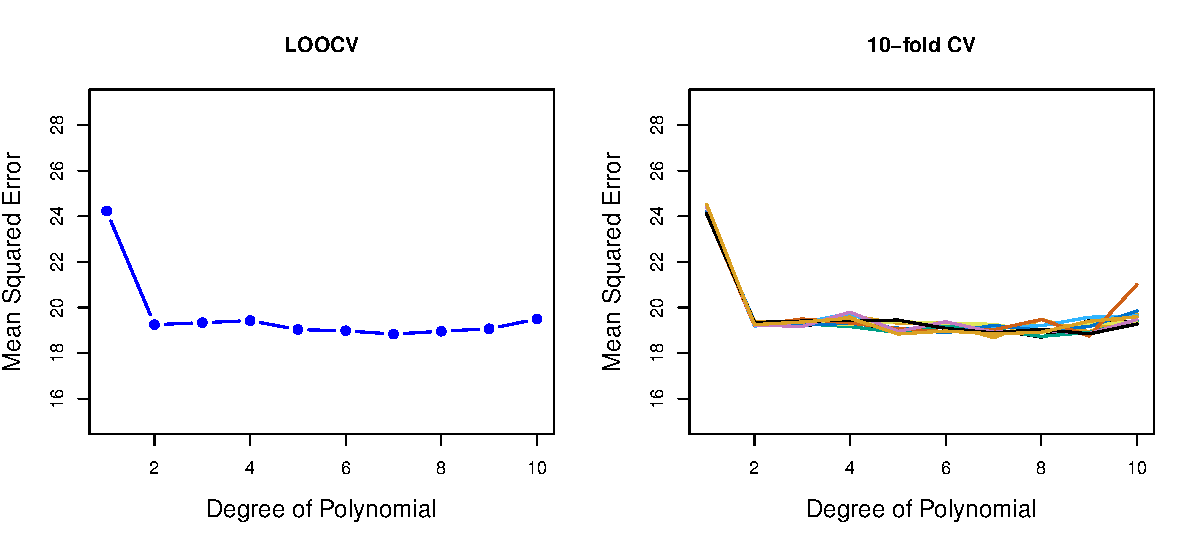
\includegraphics[width=\textwidth]{Figures_Chapters_1-6/Chapter5/5_4.pdf}
\scriptsize Source: ISLR2 Figure 5.4
\end{frame}


\begin{frame}{Cross-Validation}
To prevent ''information leakage'' from training to test or validation data:
\begin{block}{Important}
\begin{itemize}
  \item Initial analysis and predictor/feature selection must be done for each training set
  \item Data pre-processing (centering, scaling, outlier removal, etc.) must be done on each training set
\end{itemize}
\end{block}
\end{frame}


\end{document}
